\documentclass{report}
\usepackage[utf8]{vietnam}
\usepackage{amsmath}
\usepackage{graphicx}
\usepackage{float}
\usepackage{setspace}
\usepackage{fancyhdr}
\usepackage{indentfirst}
\usepackage{amsmath}
\usepackage{amsfonts}
\usepackage{amssymb}
\usepackage{wrapfig}
\usepackage{multirow}
\usepackage{pdflscape}
\usepackage{array}
\usepackage{longtable}
\usepackage{url}
\usepackage{wrapfig}
\usepackage{hyperref}
\usepackage{subfig}
\usepackage{mathptmx}
\usepackage{amsmath,amsxtra,amssymb,latexsym, amscd,amsthm}
\usepackage[left=3.50cm, right=2.00cm,top=3.50cm, bottom=3.00cm]{geometry}
\newcommand\tab[1][1.25cm]{\hspace*{#1}}

\begin{document}
\begin{center}
	\pagenumbering{gobble}
	\fontsize{14}{20}\selectfont
	\textsc{TỔNG LIÊN ĐOÀN LAO ĐỘNG VIỆT NAM\\ 
		\textbf{TRƯỜNG ĐẠI HỌC TÔN ĐỨC THẮNG\\} 
		\textbf{KHOA CÔNG NGHỆ THÔNG TIN}}
	
	\vspace{0.08cm}
	\begin{figure}[htp]
		\begin{center}
			
\includegraphics[width=5cm]{images/TĐT_logo.png}
		\end{center}
	\end{figure}
	
	\fontsize{15}{20}\selectfont\textbf{BÁO CÁO CUỐI KỲ MÔN\\HỆ THỐNG THƯƠNG MẠI THÔNG MINH\\}
	
	\vspace{2cm}
	\fontsize{24}{20}\selectfont\textbf{BANK MARKETING DATA SET}
\end{center}
\vspace{1.5cm}

\begin{flushright}
	\setstretch{1.5}
	\fontsize{14}{20}\selectfont
	\textit{Người hướng dẫn}: \textbf{TS. DƯƠNG HỮU PHÚC}\\
	\textit{Người thực hiện}:
	\textbf{NGUYỄN HOÀNG QUANG NHẬT - 51800220}\\
	\textbf{NGUYỄN THỊ HỒNG HƯƠNG - 51800284}\\
	\textbf{ĐINH TIẾN BÌNH - 51800525}\\
	\textit{Lớp}: \textbf{18050301, 18050402}\\
	\textit{Khóa}: \textbf{22}\\
\end{flushright}
\vspace{2cm}
\begin{center}
	\fontsize{14}{20}\selectfont
	\textbf{THÀNH PHỐ HỒ CHÍ MINH, NĂM 2021}
\end{center}
\pagebreak

%----------------------------------------------------------------------------------------

\begin{center}
	\pagenumbering{gobble}
	\fontsize{14}{20}\selectfont
	\textsc{TỔNG LIÊN ĐOÀN LAO ĐỘNG VIỆT NAM\\ 
		\textbf{TRƯỜNG ĐẠI HỌC TÔN ĐỨC THẮNG\\} 
		\textbf{KHOA CÔNG NGHỆ THÔNG TIN}}
	
	\vspace{0.08cm}
	\begin{figure}[htp]
		\begin{center}
			
\includegraphics[width=5cm]{images/TĐT_logo.png}
		\end{center}
	\end{figure}
	
	\fontsize{15}{20}\selectfont\textbf{BÁO CÁO CUỐI KỲ MÔN\\HỆ THỐNG THƯƠNG MẠI THÔNG MINH\\}
	
	\vspace{2cm}
	\fontsize{24}{20}\selectfont\textbf{BANK MARKETING DATA SET}
\end{center}
\vspace{1.5cm}

\begin{flushright}
	\setstretch{1.5}
	\fontsize{14}{20}\selectfont
	\textit{Người hướng dẫn}: \textbf{TS. DƯƠNG HỮU PHÚC}\\
	\textit{Người thực hiện}:
	\textbf{NGUYỄN HOÀNG QUANG NHẬT}\\
	\textbf{NGUYỄN THỊ HỒNG HƯƠNG}\\
	\textbf{ĐINH TIẾN BÌNH}\\
	\textit{Lớp}: \textbf{18050301, 18050402}\\
	\textit{Khóa}: \textbf{22}\\
\end{flushright}
\vspace{2cm}
\begin{center}
	\fontsize{14}{20}\selectfont
	\textbf{THÀNH PHỐ HỒ CHÍ MINH, NĂM 2021}
\end{center}
\pagebreak

%------------------------------------------------------------------------------------------

\pagestyle{fancy}
\fancyhf{}
\chead{\thepage}
\renewcommand{\headrulewidth}{0pt}
\begin{center}
	\pagenumbering{roman}\setcounter{page}{1}
	\fontsize{16}{20}\selectfont
	\textbf{LỜI CẢM ƠN\\} 
\end{center}
	\setstretch{1.5}
	\fontsize{13}{15}\selectfont
	\paragraph{}
    Chúng em xin chân thành cảm ơn TS Dương Hữu Phúc đã cung cấp những kiến thức vô cùng quý báu về môn học. Trong suốt quá trình giảng dạy, thầy đã nhiệt tình chỉ bảo chúng em rất nhiều để có thể tiến hành thực hiện bài báo cáo này. \\
    \indent Sau khoảng thời gian học tập, với những kiến thức đã tiếp thu được từ thầy song vẫn còn mặt hạn chế từ phía kiến thức cũng như kĩ năng thực hành nên bài báo cáo này không thể tránh khỏi sai và thiếu sót.\\
    \indent Một lần nữa nhóm chúng em xin cảm ơn thầy và mong nhận được những đóng góp quý giá từ thầy để bài báo cáo được chỉnh chu và hoàn thiện hơn nữa.
\pagebreak

\begin{center}
	\setstretch{1.0}
	\fontsize{16}{20}\selectfont
	\textbf{ĐỒ ÁN ĐƯỢC HOÀN THÀNH}\\
	\textbf{TẠI TRƯỜNG ĐẠI HỌC TÔN ĐỨC THẮNG\\} 
\end{center}
\setstretch{1.5}
\fontsize{13}{15}\selectfont
\paragraph{}
Chúng tôi xin cam đoan đây là sản phẩm đồ án của riêng  chúng tôi và được sự hướng dẫn của TS Dương Hữu Phúc. Các nội dung nghiên cứu, kết quả trong đề tài này là trung thực và chưa công bố dưới bất kỳ hình thức nào trước đây. Những số liệu trong các bảng biểu phục vụ cho việc phân tích, nhận xét, đánh giá được chính tác giả thu thập từ các nguồn khác nhau có ghi rõ trong phần tài liệu tham khảo.
\paragraph{}
Ngoài ra, trong đồ án còn sử dụng một số nhận xét, đánh giá cũng như số liệu của các tác giả khác, cơ quan tổ chức khác đều có trích dẫn và chú thích nguồn gốc.
\paragraph{}
\textbf{Nếu phát hiện có bất kỳ sự gian lận nào chúng tôi xin hoàn toàn chịu trách nhiệm về nội dung đồ án của mình.} Trường đại học Tôn Đức Thắng không liên quan đến những vi phạm tác quyền, bản quyền do chúng tôi gây ra trong quá trình thực hiện (nếu có).

\begin{flushright}
   \emph{TP.Hồ Chí Minh, ngày \hspace{0.5cm}tháng \hspace{0.5cm}năm \hspace{0.5cm}}\\
    {\emph{Tác giả}} \hskip 2cm \quad\ \\
    {\emph{(kí và ghi rõ họ tên)}} \hskip 1cm \quad\ \\
    \vspace*{1.5cm}
{\emph{Nguyễn Thị Hồng Hương}} \hskip 1cm \quad\ \\
    \vspace*{1.5cm}
{\emph{Đinh Tiến Bình}} \hskip 2cm \quad\ \\
    \vspace*{1.5cm}
{\emph{Nguyễn Hoàng Quang Nhật}} \hskip 0.5cm \quad\ 

\end{flushright}
\pagebreak

%-----------------------------------------------------------------------------------------

\begin{center}
	\setstretch{1.0}
	\fontsize{16}{20}\selectfont
	\textbf{PHẦN NHẬN XÉT VÀ ĐÁNH GIÁ CỦA GIẢNG VIÊN}\\
\end{center}
\setstretch{1.5}
\fontsize{13}{14}\selectfont
\textbf{Phần xác nhận của GV hướng dẫn}\\
\rule{16cm}{1pt}\\
\rule{16cm}{1pt}\\
\rule{16cm}{1pt}\\
\rule{16cm}{1pt}\\
\rule{16cm}{1pt}\\
\rule{16cm}{1pt}\\
\rule{16cm}{1pt}\\
\begin{flushright}
	TP. Hồ Chí Minh, ngày \tab[1cm] tháng \tab[1cm] năm \tab[1cm]\tab \\
	(ký tên và ghi rõ họ tên)\tab[2cm] \\
	\vspace{2cm}
\end{flushright}
\setstretch{1.5}
\fontsize{13}{14}\selectfont
\textbf{Phần đánh giá của GV chấm bài}\\
\rule{16cm}{1pt}\\
\rule{16cm}{1pt}\\
\rule{16cm}{1pt}\\
\rule{16cm}{1pt}\\
\rule{16cm}{1pt}\\
\rule{16cm}{1pt}\\
\rule{16cm}{1pt}\\
\begin{flushright}
	TP. Hồ Chí Minh, ngày \tab[1cm] tháng \tab[1cm] năm \tab[1cm]\tab \\
	(ký tên và ghi rõ họ tên)\tab[2cm] \\
	\vspace{1.5cm}
\end{flushright}
\pagebreak

\begin{center}
	\setstretch{1.0}
	\fontsize{16}{20}\selectfont
	\textbf{TÓM TẮT}\\
	\end{center}
	\fontsize{13}{15}\selectfont
	\paragraph{}
	Ngày nay, dữ liệu chính là vua. Sử dụng dữ liệu với các mục đích khác nhau cho tác dụng to lớn đối với doanh nghiệp thương mại. Ngoài ra, một trong những cách mà tổ chức doanh nghiệp có thể thực hiện khi đứng trên thị trường là nắm bắt và kiểm tra thành thạo thông tin khách hàng để phát triển hơn nữa trải nghiệm của khách hàng. Bài báo cáo này thu thập tập dữ liệu được thu thập từ trang UCI Machine Learning Repository. Thông tin được xác định với các chiến dịch tiếp thị ngân hàng của các cơ sở cuộc gọi. Mục tiêu chính là trực quan hóa dữ liệu trên Tableau và thử nghiệm xem liệu khách hàng có quyết định đăng ký dịch vụ gửi tiền có kỳ hạn hay không. Bên cạnh đó báo cáo có trình bày sơ lược lý thuyết một số thuật toán như Naive Bayes, Decision Tree, Support Vector Machine, Logistic Regression và K-Nearest Neighbor và tiến hành đưa ra các xác suất dự đoán dựa trên tập dữ liệu này.


%-------------------------------------------------------------------------------------------------------------
\setstretch{1.5}
\fontsize{13}{15}\selectfont

%-------------------------------------------------------------------------------------------------------------
\pagebreak
%-------------------------------------------------------------------------------------------------------------


\fontsize{13}{20}\selectfont
\tableofcontents
\pagebreak

%\fontsize{13}{20}\selectfont
%\listoftables
%\pagebreak

\fontsize{13}{20}\selectfont
\listoffigures
\pagebreak

%-------------------------------------------------------------------------------------------------------------
%---------------Chương 1 -----------------------
\pagenumbering{arabic}\setcounter{page}{1}
\fontsize{16}{10}\selectfont
\chapter{TỔNG QUAN ĐỀ TÀI}
\fontsize{14}{10}\selectfont
\section{Giới thiệu đề tài}
 \fontsize{13}{14}\selectfont
 Một trong những tổ chức ngân hàng Bồ Đào Nha đã thực hiện một chiến dịch tiếp thị dựa trên các cuộc điện thoại từ năm 2008 đến năm 2010. Các hồ sơ về nổ lực trong chiến dịch tiếp thị của họ có sẵn dưới dạng tập dữ liệu. Bài báo cáo này sẽ áp dụng các thuật toán học máy để phân tích tập dữ liệu dự đoán xem khách hàng có đăng ký tiền gửi có hạn không, cũng nhằm tìm ra các chiến thuật hiệu quả nhất giúp ngân hàng trong chiến dịch tiếp theo thuyết phục thêm nhiều khách hàng đăng ký gửi tiền có kỳ hạn. Tập dữ liệu chứa các tính năng phân loại và số khác nhau với 41188 mẫu dữ liệu. Dữ liệu được gắn nhãn. Mục tiêu là dự đoán liệu khách hàng có đăng ký tiền gửi có kỳ hạn hay không. Xử lý trước dữ liệu được thực hiện cùng với phân tích dữ liệu phù hợp. Kết quả của các thuật toán khác nhau sẽ được so sánh.
 
\fontsize{14}{10}\selectfont
\section{Phát biểu bài toán}
 \fontsize{13}{14}\selectfont
Trong một môi trường thông tin điện tử phát triển mạnh mẽ như ngày nay thì các tổ chức hàng ngày thiết lập các bộ dữ liệu, tìm hiểu và kết hợp chúng để đưa ra những quyết định hiệu quả để cải thiện thương mại. Việc công nghệ đi kèm với lượng dữ liệu dồi dào đóng vai trò then chốt thì khả năng quyết định nhanh chóng và chuẩn xác là một lợi thế cạnh tranh vô cùng quan trọng. Hệ thống thương mại thông minh (BI - Business Intelligence) mang đến lợi ích giúp người dùng đưa ra những quyết định đúng đắn, gia tăng giá trị của doanh nghiệp nói chung. Đặc biệt là trong ngành ngân hàng, việc phân tích, xử lý và khai thác những nguồn thông tin khổng lồ có được từ khách hàng giúp đưa ra các chiến lược tiếp thị thu hút khách hàng cũng như tiềm năng dịch vụ hay rủi ro của ngân hàng. Tốc độ thành công của tiếp thị ngân hàng phụ thuộc vào kết quả và sự lựa chọn để đưa ra các dự đoán và chiến lược chính xác hơn.\\
\indent Từ thực tế đó, trên cơ sở nhu cầu ngày càng cao của việc đưa ra các chiến lược tiếp thị trong ngành ngân hàng thì chúng em đã quyết định chọn đề tài "Bank Marketing Data Set" nhằm nghiên cứu và tìm hiểu về quá trình xử lý tập dữ liệu của một ngân hàng để dự đoán xem khách hàng có đăng ký dịch vụ gửi tiền có kỳ hạn hay không trong chiến dịch tiếp thị này.
 
 
\fontsize{14}{10}\selectfont
\section{Mục tiêu chọn đề tài}
     \fontsize{13}{14}\selectfont
Dự đoán, đưa ra các xác suất, tỉ lệ mà khách hàng tại ngân hàng có quyết định đăng ký gửi một khoản tiền có thời hạn hay không.
\begin{itemize}
    \item Áp dụng các thuật toán học máy xử lý và phân tích dữ liệu.
    \item Tìm hiểu thuật toán hồi quy logistics, K-Nearest Neighbors, Support Vector Machine, Decision Tree và Naive Bayes để xác định.
    \item Trực quan hóa tập dữ liệu trên Tableau.
\end{itemize}

\fontsize{14}{10}\selectfont
\section{Phạm vi đề tài}
 \fontsize{13}{14}\selectfont
  \begin{enumerate}
                \item[- ] Sử dụng 5 thuật toán là KNN, Decision Tree, hồi quy logistic, SVM và Naive Bayes.
                \item[- ] Dùng Tableau để thể hiện đồ thị trực quan.

    \end{enumerate} 
\fontsize{14}{10}\selectfont
\section{Cấu trúc báo cáo}
 \fontsize{13}{14}\selectfont
Bài báo cáo gồm có 6 chương:\\\tab
 \textit{Chương 1 – Tổng quan đề tài}: Chương này giới thiệu đề tài, trình bày đặt vấn đề bài toán dẫn nhập mục tiêu, phạm vi nghiên cứu và cấu trúc của báo cáo.\\\tab
 \textit{Chương 2 – Tổng quan giải thuật}: Chương này trình bày tổng quan các lý thuyết giải thuật, và thực nghiệm giải thuật đó trên đề tài.\\\tab
 \textit{Chương 3 – Dữ liệu thực nghiệm}: Chương này trình bày chi tiết về tập dữ liệu sử dụng trong đề tài, trực quan hóa tập dữ liệu đó bằng đồ thị trên Tableau và cách xử lý dữ liệu.\\\tab
 \textit{Chương 4 – Thực nghiệm}: Chương này trình bày các kết quả với các thuật toán giới thiệu ở chương 2 và đưa ra nhận xét.\\\tab
 \textit{Chương 5 – Kết luận}: Chương này trình bày những gì đã làm được và chưa làm được so với mục tiêu ban đầu đặt tra và nêu hướng phát triển trong tương lai.\\\tab
 \textit{Chương 6 – Tài liệu tham khảo}: Chương này tổng hợp các tài liệu tham khảo và dẫn đến các đường dẫn đó.


%-------------------------------------------------------------------------------------------------------------
%---------------Chương 2 -----------------------
\fontsize{16}{10}\selectfont
\chapter{TỔNG QUAN GIẢI THUẬT}
\fontsize{14}{10}\selectfont
\section{Thuật toán K-Nearest Neighbors (KNN)}
\subsection{\textit{Cơ sở lý thuyết}}
    \fontsize{13}{14}\selectfont
    K-nearest neighbor là một trong những thuật toán supervised-learning đơn giản nhất (mà hiệu quả trong một vài trường hợp) trong Machine Learning. KNN là thuật toán tìm đầu ra của một điểm dữ liệu mới bằng cách chỉ dựa trên thông tin của K điểm dữ liệu trong training set gần nó nhất (K-lân cận).
    \begin{enumerate}
                \item[- ] Ứng dụng:  Thuật toán KNN có nhiều ứng dụng trong ngành ngân hàng gồm xác định xem khách hàng chậm trả các khoản vay, khách hàng có đăng ký gửi tiền hạn hay không; trong đầu tư như dự đoán phá sản, dự đoán giá cổ phiếu, phân bổ xếp hạng tín dụng trái phiếu doanh nghiệp, tạo ra chỉ số vốn và trái phiếu tùy chỉnh.
                \item [- ] Ưu điểm:
                    \begin{itemize}
                        \item Thuật toán đơn giản, dễ dàng triển khai.
                        \item Độ phức tạp tính toán của quá trình training nhỏ.
                        \item Việc dự đoán kết quả của dữ liệu mới rất đơn giản.
                        \item Xử lý tốt với tập dữ liệu bị nhiễu.
                    \end{itemize}
                \item [- ] Nhược điểm:
                    \begin{itemize}
                        \item KNN bị nhiễu dễ đưa ra kết quả không chính xác khi K nhỏ.
                        \item KNN là một thuật toán mà mọi tính toán đều nằm ở khâu test. Việc tính khoảng cách tới từng điểm dữ liệu trong training set sẽ tốn rất nhiều thời gian.
                        \item Độ phức tạp càng tăng khi k càng lớn.
                    \end{itemize}
                \item [- ] Ý tưởng thuật toán:
        Thuật toán KNN cho rằng những dữ liệu tương tự nhau sẽ tồn tại gần nhau trong một không gian, từ đó công việc của ta là sẽ tìm k điểm gần với dữ liệu cần kiểm tra nhất. Việc tìm khoảng cách giữa 2 điểm có nhiều công thức có thể sử dụng, tùy trường hợp mà chúng ta lựa chọn cho phù hợp. Đây là 3 cách cơ bản để tính khoảng cách 2 điểm dữ liệu x, y có k thuộc tính:
            \end{enumerate}
    \begin{center}
        \begin{figure}[htp]
    	\begin{center}
    		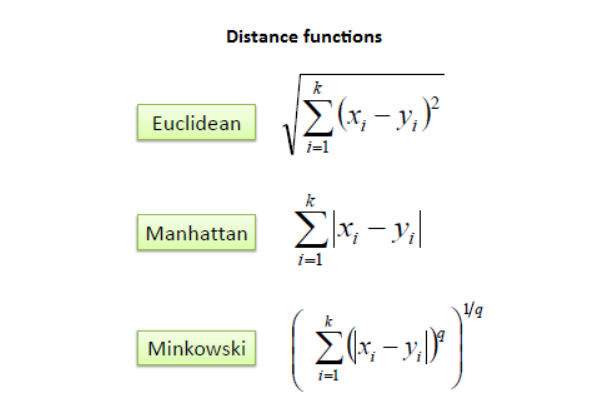
\includegraphics[width=15cm, height=8cm]{images/CT_KNN.PNG}
    	\end{center}
    		\caption{Một số công thức tính khoảng cách giữa x và y có k thuộc tính}
        \end{figure}
    \end{center}
    \indent Các bước trong KNN:
    \begin{enumerate}
        \item Ta có D là tập dữ liệu đã được gắn nhãn và A là dữ liệu chưa được phân loại.
        \item Đo khoảng cách từ A đến tất cả dữ kiệu đã được phân loại trong D.
        \item Chọn K làm khoảng cách nhỏ nhất.
        \item Kiểm tra danh sách có khoảng cách ngắn nhất và đếm số lượng lớp xuất hiện.
        \item Lấy lớp xuất hiện nhiều nhất.
        \item Lớp dữ liệu mới là lớp ở bước 5.
    \end{enumerate}
\subsection{\textit{Thực hành trên tập dữ liệu}}
    \fontsize{13}{14}\selectfont
    Lấy ra 4 biến độc lập gồm job, marital, housing và loan đã được gắn nhãn phân loại. Chọn ra 10 dữ liệu để xét:
        \begin{center}
        \begin{figure}[htp]
    	\begin{center}
    		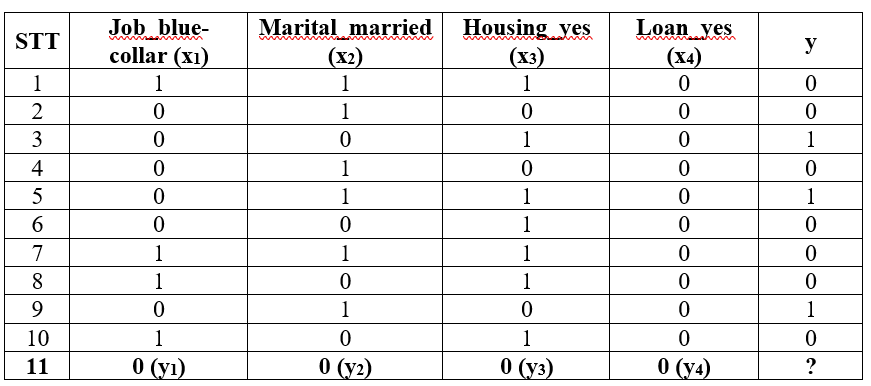
\includegraphics[width=15cm, height=7cm]{images/vd_knn.png}
    	\end{center}
    		\caption{Bảng ví dụ dữ liệu trong tập dữ liệu}
    \end{figure}
    \end{center}
    Áp dụng hàm Euclidean tính khoảng cách:
    $$D = \sqrt{(x_1 - y_1)^2 + (x_2 - y_2)^2 + (x_3 - y_3)^2 + (x_4 - y_4)^2}$$
\pagebreak
        \begin{center}
        \begin{figure}[htp]
    	\begin{center}
    		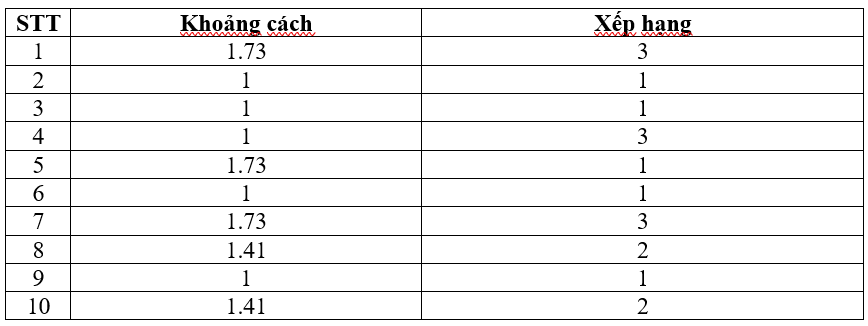
\includegraphics[width=15cm, height=7cm]{images/kq_knn.png}
    	\end{center}
    		\caption{Kết quả tính khoảng cách}
    \end{figure}
    \end{center}
    \indent Chọn K=5, ta được:
    \begin{center}
        \begin{figure}[htp]
    	\begin{center}
    		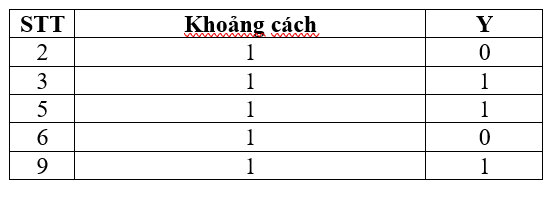
\includegraphics[width=15cm, height=6cm]{images/kqknn.png}
    	\end{center}
    		\caption{Kết quả thu được lớp dữ liệu mới}
    \end{figure}
    \end{center}
  $\Rightarrow$ trong 5 dữ liệu mới được chọn, nhãn 1 chiếm đa số vậy dữ liệu số 11 được phân vào lớp 1.
 
\fontsize{14}{10}\selectfont
\section{Thuật toán hồi quy logistic}
\subsection{\textit{Cơ sở lý thuyết}}
    \fontsize{13}{14}\selectfont
    Hồi quy từ lâu đã trở thành một phần không thể thiếu trong Data analysis liên quan đến việc tìm hiểu và phân tích mối quan hệ giữa các đối tượng nghiên cứu thể hiện qua biến mục tiêu (biến y) và các biến độc lập (biến giải thích - các biến x).
        \begin{enumerate}
                \item[- ]\textbf{ Ứng dụng:} 
                    \begin{itemize}
                        \item Dự đoán phân loại email có spam hay không
                        \item Dự đoán khả năng trả nợ của khách hàng.
                        \item Dự đoán khả năng mua sản phẩm hay là đăng ký dịch vụ,...
                    \end{itemize}
                \item [- ] \textbf{ Phương trình hồi quy logistic:}
\begin{enumerate}
        \item [- ] Probability (p); là xác suất của một biến cố trong một thời gian (p sẽ dao động trong khoảng từ 0 đến 1).
        \item [- ] odds: là tỷ số giữa xác suất biến cố xảy ra chia cho xác suất biến cố không xảy ra. Odds được xem là một biến liên tục, giá trị của odds không nhất thiết phải nằm tròn khoản từ 0 đến 1 và giá trị của odds bằng 1 khi và chỉ khi p = 0.5. Để tính odds chúng ta áp dụng công thức: $odd = \frac{p}{1 - p}$
        \item [- ] odds ratio: là tỷ số giữa 2 odd vầ được xác định bằng công thứ; $ \frac{odd_1}{odd_2} = \frac{P(X,Y)P(\overline{X},\overline{Y})}{P(X,\overline{Y}P(\overline{X},Y)}$
        \vspace{0.2cm}\tab\textit{\textbf{Ví dụ:} Xét trường hợp 5 người cùng đến xét nghiệm ung thư phổi và kết quả trả về là 1 người trong số họ mắc bệnh.}\vspace{0.2cm}
        \newline\tab\quad Ta có: $p = \frac{1}{5} = 0.2$\\
        \vspace{0.2cm}\newline\tab\quad$\Rightarrow odds = \frac{p}{1 - p} = \frac{0.2}{1-0.2} = 0.25$
        \item [- ] logit chính là $\log(odds)$ và được xác định bằng công thức: \\\tab\textbf{$logit(p) = \log(odds) = \log(\frac{p}{1 - p})$}
        \item [- ] Nếu gọi X là biến tiên lượng và p là xác suất của một biến cố (outcome) thì mô hình hồi quy logistic sẽ được phát biểu như sau:
        \vspace{0.2cm}\newline\tab[6cm] $logit(p) = \alpha + \beta X$ \newline\tab[5cm] hay: \vspace{0.2cm}\newline\tab[6cm] $\log(\frac{p}{1 - p}) = \alpha + \beta X$
        \item [- ] Phương trình tổng quát để ước lượng xác suất dạng đa biến như sau:
        \vspace{0.2cm}\newline\tab[2cm] $\hat{y} = $ Ước lượng P( y = 1 $\mid x_1, x_2,...,x_p) = \frac{e^{\alpha + \beta_1x_1 + \beta_2x_2 + ... + \beta_px_p}}{1 + e^{\alpha + \beta_1x_1 + \beta_2x_2 + ... + \beta_px_p}}$
        Trong đó:
        \begin{itemize}
            \item $\alpha$ là hệ số chặn (intercept). Giá trị của z khi tất cả các biến độc lập bằng 0 (X=0).
            \item $\beta$ là hệ số hồi qui (regression cofficients) của các  yếu tố nguy cơ (còn gọi là biến độc lập) x1, x2,…, xk. Hệ số hồi qui cho biết độ mạnh cũng như chiều của sự ảnh hưởng của các yếu tố nguy cơ đến xác suất xảy ra sự kiện nghiên cứu. Nếu hệ số hồ qui dương thì yếu tố nguy cơ làm tăng khả năng (xác suất) xảy ra của sự kiện nghiên cứu và ngược lại.
        \end{itemize}
    \end{enumerate}
\end{enumerate}
    
\subsection{\textit{Thực hành trên tập dữ liệu}}
    \fontsize{13}{14}\selectfont
            \begin{enumerate}
                \item[- ] Để dự đoán dữ liệu trong mô hình Logistic Regression thì ta phải tính xác suất để xác định ngưỡng để cho biết dữ liệu đó thuộc nhãn 0 hay 1 thông qua hàm sigmoid.
                \item[- ] Nếu kết quả trả về của hàm Sigmoid đó >= 0.5 thì sẽ là nhãn 1 còn < 0.5 thì sẽ là nhãn 0.
                \item[- ] Ví dụ: một khách hàng có thuộc tính {age:40, martial: married, loan:yes, default: no…..} thì sẽ được tính qua hàm sigmod có dạng là:  
                $$ Y = \frac{1}{1 + e^{\ -z}} $$ 
                \begin{itemize}
                \item Z= W0 + W1.age + W2.married + W3.loan+ ...
                \item Giả sử như Y < 0.5 thì ta sẽ kết luẫn khách hàng này thuộc nhãn 0 (y=0) nghĩa là khách hàng này không đăng ký tiền gửi có kỳ hạn.
                \end{itemize}
            \end{enumerate}

\fontsize{14}{10}\selectfont
\section{Thuật toán Naive Bayes}
\subsection{\textit{Cơ sở lý thuyết}}
    \fontsize{13}{14}\selectfont
    Naive Bayes Classification (NBC) là một thuật toán phân loại dựa trên tính toán xác suất áp dụng định lý Bayes. Theo định lý Bayes, ta có công thức tính xác suất ngẫu nhiên của sự kiện yy khi biết xx như sau :
     $$P(y \mid x)=\frac {P(x \mid y) P(y)} {P(x)} $$
    \indent Giả sử ta phân chia sự kiện x thành n thành phần khác nhau x1 ,x2 ....,xn. Naive Bayes theo đúng như tên gọi dựa vào một giả thiết x1 ,x2 ....,xn  là các thành phần độc lập với nhau. Từ đó ta có thể tính được:
    $$P(x \mid y)=P(x_1 \cap x_2 \cap ... \cap x_n \mid y) = P(x_1 \mid y)P(x_2 \mid y)(x_3 \mid y)...P(x_n \mid y) $$
    \indent Do đó ta có:
    $$ P(y \mid x) \propto P(y) \prod_{i=1}^{n}P(x_i \mid y) $$
    Trong đó $ \propto$ là phép tỉ lệ thuận.
 \begin{enumerate}
                \item[- ] \textbf{Các mô hình thuật toán Naive Bayes}:
                    \begin{itemize}
                        \item \textbf {\textit{Mô hình Bernoulli:}} mô hình này, các feature vector là các giá trị nhị phân 0, 1. Trong đó 1 thể hiện từ có xuất hiện trong dữ liệu , 0 thể hiện từ đó không xuất hiện trong dữ liệu. Xác suất $P (x_i \mid y )$ được tính bằng :
                        $$ P(x_i \mid y)=P(i \mid y).x_i+(1-P(i \mid y)).(1-x_i)$$
                        Với $P (x_i \mid y )$ tỉ lệ số lần từ $x_i$ xuất hiện trong toàn bộ tập training data có nhãn y.
                        \item \textbf{\textit{Mô hình Multinomial: }}Ở mô hình này, các feature vector là các giá trị số tự nhiên mà giá trị thể hiện số lần từ đó xuất hiện trong văn bản. Ta tính xác suất từ xuất hiện trong dữ liệu $P (x_i \mid y )$ như sau:
                        $$P(x_i \mid y)=\frac{N_i}{N_c}$$
                        Với $N_i$ là tổng số lần từ $x_i$ xuất hiện trong văn bản, $N_c$ là tổng số lần từ của tất cả các từ X1,....Xn xuất hiện trong dữ liệu.
                    \end{itemize}
\end{enumerate}

\subsection{\textit{Thực hành trên tập dữ liệu}}
    \fontsize{13}{14}\selectfont
  \begin{center}
        \begin{figure}[htp]
    	\begin{center}
    		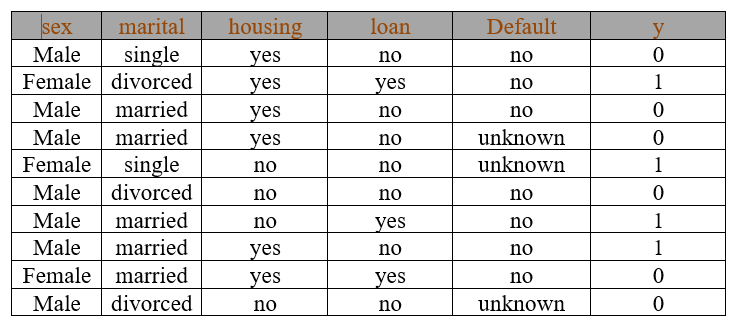
\includegraphics[width=15cm, height=7cm]{images/Nb_ex.PNG}
    	\end{center}
    		\caption{Bảng ví dụ dữ liệu trong tập dữ liệu}
    \end{figure}
    \end{center}
   P(y=0)=6/10 và P(y=1)=4/10\\
       \indent Ví dụ như cần dư đoán xem khách hàng có các thuộc tính {sex:female; marital:married; housing:yes; loan:no; default:unknown} để biết người đó có đăng kí tiền gửi có kì hạn hay không thì ta sẽ làm như sau:
  \pagebreak
   \begin{center}
        \begin{figure}[htp]
    	\begin{center}
    		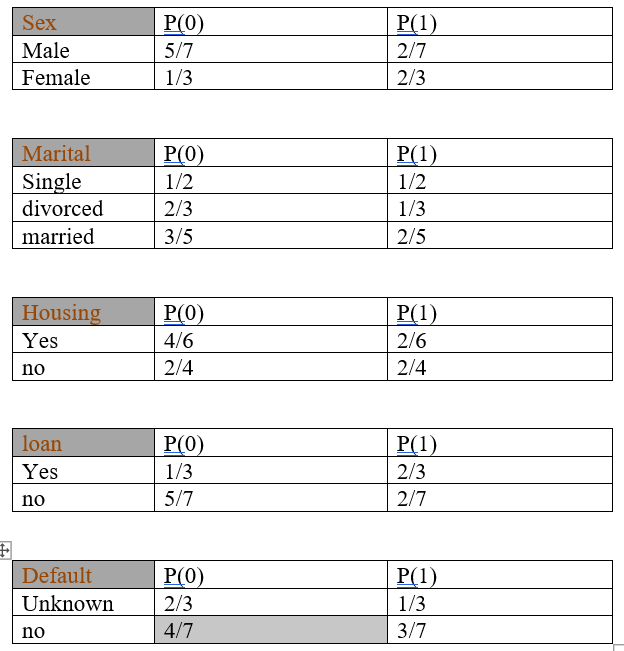
\includegraphics[width=10cm, height=9cm]{images/vd_nb.PNG}
    	\end{center}
    		\caption{Bảng tính toán dự đoán P}
    \end{figure}
    \end{center}

    \begin{enumerate}
                \item[- ] Tính xác suất với P(y=1): \\
                P(1)*P(female|1)*P(married|1)*P(yes|1)*P(no|1)*(unknown|1)\\
=4/10*2/3*2/5*2/6*2/7*1/3 = 0.003
                \item[- ] Tính xác suất với P(y=0): \\
            P(0)*P(female|0)*P(married|0)*P(yes|0)*P(no|0)*(unknown|0)\\
=6/10*1/3*3/5*4/6*5/7*2/3 = 0.038
\item [$\Rightarrow$] Ta thấy 0.038 > 0.003 do đó khách hàng này sẽ có y = 0, nghĩa là khách hàng này không đăng kí tiền gửi có kỳ hạn.
     \end{enumerate}           

\fontsize{14}{10}\selectfont
\section{Thuật toán Support Vector Machine (SVM)}
\subsection{\textit{Cơ sở lý thuyết}}
    \fontsize{13}{14}\selectfont
SVM là một thuật toán giám sát, nó có thể sử dụng cho cả việc phân loại hoặc đệ quy. Tuy nhiên nó được sử dụng chủ yếu cho việc phân loại. Trong thuật toán này, chúng ta vẽ đồ thị dữ liệu là các điểm trong n chiều với giá trị của mỗi tính năng sẽ là một phần liên kết. Sau đó chúng ta thực hiện tìm "đường bay" (hyper-plane) phân chia các lớp. Hyper-plane nó chỉ hiểu đơn giản là 1 đường thẳng có thể phân chia các lớp ra thành hai phần riêng biệt.\\
\indent Margin trong SVM là khoảng cách giữa siêu phẳng đến 2 điểm dữ liệu gần nhất tương ứng với các phân lớp. Ví dụ quả táo quả lê đặt trên mặt bàn, margin chính là khoảng cách giữa cây que và hai quả táo và lê gần nó nhất. Điều quan trọng ở đây đó là phương pháp SVM luôn cố gắng cực đại hóa margin này, từ đó thu được một siêu phẳng tạo khoảng cách xa nhất so với 2 quả táo và lê. Nhờ vậy, SVM có thể giảm thiểu việc phân lớp sai (misclassification) đối với điểm dữ liệu mới đưa vào.\\
\indent Phương thức Kernel: 
    \begin{enumerate}
                \item[- ]Ý tưởng:
                \begin{itemize}
                    \item Định nghĩa K: X x Y $ \rightarrow \mathbb {R} $ được gọi là kernel với: $$ \Phi(x). \Phi(y) = K(x,y)$$
                    \item K thường được hiểu là đại lượng đo độ tương đồng.
                \end{itemize}
                \item[- ] Kernel là các hàm cho trước x, y trả về $ \Phi(x), \Phi(y)$. Điều này có nghĩa là chúng ta có thể biến đổi các vectơ đặc trưng thành chiều vô hạn và vẫn không có thêm bất kỳ tính toán nào để tính các điểm chấm.
    \end{enumerate}
\subsection{\textit{Thực hành trên tập dữ liệu}}
    \fontsize{13}{14}\selectfont
    \begin{enumerate}
                \item[- ] Để dự đoán được dữ liệu bằng phương pháp SVM thì ta phải giải phương trình W.X + B = 0 để tìm ra được đường phân cách giữa nhãn 0 và nhãn 1 trong y.
                \item[- ] Tiếp theo đó ta sẽ tìm Margin là đường mở rộng ra từ phương trình W.X + B = 0 sao cho nó càng rộng càng tốt. các biên của margin sẽ chạm vào các điểm đầu tiên của 2 nhãn và điểm đó sẽ được gọi là support vector.
                \item[- ]Để kiểm tra xem dữ liệu cần dự đoán thuộc nhãn 0 hay 1 thì ta sẽ tính phương trình W.X + B cho dữ liệu đó nếu cái phương trình W.X + B này lớn hơn hoặc bằng 1 thì nó thuộc nhãn 1 còn bé hơn hoặc bằng -1 thì nó sẽ thuộc nhãn 0.
                \item[- ] Ví dụ: khách hàng có các thuộc tính {age: 55, sex:male, martial:single ....} thì sau khi tính phương trình W.X + B >= 1 từ đó ta sẽ kết luận khách hàng này có y =1 tức là có đăng ký tiền gửi có kỳ hạn.
    \end{enumerate}

\fontsize{14}{10}\selectfont
\section{Thuật toán Decision Tree}
\subsection{\textit{Cơ sở lý thuyết}}
    \fontsize{13}{14}\selectfont
    Cây quyết định (Decision tree) là một cây phân cấp có cấu trúc được dùng để phân lớp các đối tượng dựa vào dãy các luật. Các thuộc tính của đối tượng có thể thuộc các kiểu dữ liệu khác nhau như Nhị phân (Binary) , Định danh (Nominal), Thứ tự (Ordinal), Số lượng (Quantitative) trong khi đó thuộc tính phân lớp phải có kiểu dữ liệu là Binary hoặc Ordinal. Tóm lại, cho dữ liệu về các đối tượng gồm các thuộc tính cùng với lớp (classes) của nó, cây quyết định sẽ sinh ra các luật để dự đoán lớp của các dữ liệu chưa biết.
    \begin{enumerate}
        \item[- ]Ưu điểm: 
        \begin{itemize}
        \item Mô hình sinh ra các quy tắc dễ hiểu cho người đọc, tạo ra bộ luật với mỗi nhánh lá là một luật của cây.
        \item Dữ liệu đầu vào có thể là là dữ liệu missing, không cần chuẩn hóa hoặc tạo biến giả.
        \item Có thể làm việc với cả dữ liệu số và dữ liệu phân loại.
        \item Có thể xác thực mô hình bằng cách sử dụng các kiểm tra thống kê.
        \item Có khả năng là việc với dữ liệu lớn.
        \end{itemize}
        \item[- ]Nhược điểm: 
        \begin{itemize}
        \item Mô hình cây quyết định phụ thuộc rất lớn vào dữ liệu của bạn. Thạm chí, với một sự thay đổi nhỏ trong bộ dữ liệu, cấu trúc mô hình cây quyết định có thể thay đổi hoàn toàn.
        \item Cây quyết định hay gặp vấn đề overfitting.
        \end{itemize}
        \item [- ] \textbf{Entropy: } là thuật ngữ thuộc Nhiệt động lực học, là thước đo của sự biến đổi, hỗn loạn hoặc ngẫu nhiên. Năm 1948, Shannon đã mở rộng khái niệm Entropy sang lĩnh vực nghiên cứu, thống kê với một phân phối xác suất của một biến rời rạc x có thể nhận n giá trị khác nhau x1,x2,…,xn. Giả sử rằng xác suất để x nhận các giá trị này là $pi=p(x=x_i)$. Ta có công thức tổng quát sau:
        $$ Entropy(S) = \sum_{i=1}^{c} - p_i.log_2.p_i$$
        \item [- ] \textbf{Information Gain: } dựa trên sự giảm của hàm Entropy khi tập dữ liệu được phân chia trên một thuộc tính. Để xây dựng một cây quyết định, ta phải tìm tất cả thuộc tính trả về Infomation gain cao nhất. Để xác định các nút trong mô hình cây quyết định, ta thực hiện tính Infomation Gain tại mỗi nút theo trình tự sau:
        \begin{itemize}
            \item Bước 1: Tính toán hệ số Entropy của biến mục tiêu S có N phần tử với $N_c$ phần tử thuộc lớp c cho trước 
            $$ H(S) = - \sum_{c=1}^c.(N_c)/N.log(N_c)/N $$
            \item Bước 2: Tính hàm số Entropy tại mỗi thuộc tính: với thuộc tính x, các điểm dữ liệu trong S được chia ra K child node $S_1, S_2, …, S_K $ với số điểm trong mỗi child node lần lượt là $m_1,m_2,…, m_K$, ta có:
            $$H(x,S) = \sum_{k=1}^K.(m_k)/N.H(S_k) $$
            \item Bước 3: Chỉ số Gain Information được tính bằng:
            $$G(x,S) = H(S) - H(x,S)$$
            \item Công thức tổng quát:
            $$Gain(S,A) = Entropy(S) - \sum_{v \epsilon Values (A)} \frac{{\mid S_v \mid}}{{\mid S \mid}}.Entropy(S_v) $$
        \end{itemize}
        \item [- ] \textbf{Tiêu chuẩn dừng: }Trong thuật toán Decision tree, với phương pháp chia trên, ta sẽ chia mãi các node nếu nó chưa tinh khiết. Như vậy, ta sẽ thu được một tree mà mọi điểm trong tập huấn luyện đều được dự đoán đúng (giả sử rằng không có hai input giống nhau nào cho output khác nhau). Khi đó, cây có thể sẽ rất phức tạp (nhiều node) với nhiều leaf node chỉ có một vài điểm dữ liệu. Như vậy, nhiều khả năng overfitting sẽ xảy ra. Để tránh trường hợp này, ta có thể dừng cây theo một số phương pháp sau đây:
        \begin{itemize}
            \item Nếu node đó có entropy bằng 0, tức mọi điểm trong node đều thuộc một class.
            \item Nếu node đó có số phần tử nhỏ hơn một ngưỡng nào đó. Trong trường hợp này, ta chấp nhận có một số điểm bị phân lớp sai để tránh overfitting. Class cho leaf node này có thể được xác định dựa trên class chiếm đa số trong node.
            \item Nếu khoảng cách từ node đó đến root node đạt tới một giá trị nào đó. Việc hạn chế chiều sâu của tree này làm giảm độ phức tạp của tree và phần nào giúp tránh overfitting.
            \item Nếu tổng số leaf node vượt quá một ngưỡng nào đó.
            \item Nếu việc phân chia node đó không làm giảm entropy quá nhiều (information gain nhỏ hơn một ngưỡng nào đó).
        \end{itemize}
    \end{enumerate}
\subsection{\textit{Thực hành trên tập dữ liệu}}
    \fontsize{13}{14}\selectfont
    Ta có mẫu dữ liệu với các trường sau để dự đoán khách hàng có đăng ký tiền vào ngân hàng hay không với các thuộc tính sau: Sex : giới tính, Marital: Hôn nhân, Housing: Nhà ở, Loan : Tình trạng có vay hay không, Contact: Liên lạc, Default: Vỡ nợ, y : Khách hàng có đăng ký gửi tiền hay không. 
      \begin{center}
        \begin{figure}[htp]
    	\begin{center}
    		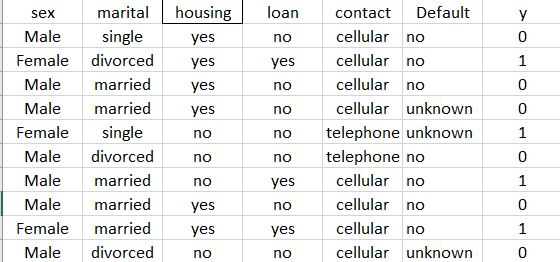
\includegraphics[scale=0.8]{images/vd_dt.png}
    	\end{center}
    		\caption{Bảng ví dụ dữ liệu trong tập dữ liệu}
    \end{figure}
    \end{center}
   $ Entropy ([4+,6-]) = -(4/10).log_2(4/10) - (6/10).log_2(6/10) = 0.97 $
  
   \begin{enumerate}
        \item[- ] Values (sex) = Male, Female \\
        $S_{Male} = [1+,6-]$ \\
        $S_{Female} = [3+,0]$ \\
        $Gain(S,sex) = Entropy(S) - (7/10).Entropy(S_{Male}) - (3/10). Entropy(S_{Female})$ = 0.97 - (7/10) * 0.59 - (3/10) * 0 = 0.4
        \item[- ] Value (marital) = single, married, divorced \\
        $S_{single} = [1+,1-] $ \\
        $S_{married} = [2+,3-]$ \\
        $S_{divorced} = [1+,2-]$ \\
        $Gain(S, marital) = Entropy(S) - (2/10).Entropy(S_{single}) - (5/10). Entropy(S_{married}) - (3/10).Entropy(S_{divorced})$ = 0.97 - (2/10) * 1 - (5/10) * 0.97 - (3/10) * 0.918 = 0.009
        \item[- ] Value (Default) = no, unknown \\
        $ S_{no} = [3+,4-]$\\
        $S_{unknown} = [1+,2-]$ \\
        $Gain(S, Default) = Entropy(S) - (7/10).Entropy(S_{no}) - (3/10).Entropy(S_{ unknown})$ = 0.97 - (7/10) *   0.985- (3/10) * 0.528 = 0.1221
        \item[- ] Value (housing) = yes , no\\
        $S_{Yes} = [2+,4-]$\\
        $S_{No}= [2+,2-]$ \\
        $Gain(S,housing) = Entropy(S) - (6/10).Entropy(S_{Yes}) - (4/10).Entropy(S_{No})$ = 0.97 - (6/10) * 0.918 - (4/10) *  1 = 0.0192
        \item[- ] Value (loan) = Yes ,no \\
        $S_{Yes} = [3+,0-]$\\
        $S_{No}= [1+,6-]$\\
        $Gain(S,loan) = Entropy(S) - (3/10).Entropy(S_{Yes}) - (6/10).Entropy(S_{No})]$ = 0.97 - (3/10) * 0 - (7/10) *  0.59 = 0.557 
        \item[- ] Value(contact) = cellular, telephone \\
        $S_{cellular} = [3+,5-]$ \\
        $S_{telephone} = [1+,1-]$\\
        $Gain(S, contact) = Entropy(S) - (8/10).Entropy(S_{cellular}) - (2/10). Entropy(S_{telephone})$ = 0.97 - (8/10) * 0.95  - (2/10) *1 = 0.01
    \end{enumerate}
    $\Rightarrow$ \textbf{Kết luận: }
    \begin{enumerate}
        \item[- ] Sau khi tính được như vậy ta thấy Gain(S,Loan)=0.557 có giá trị cao nhất nên nó sẽ đứng đầu tiên trong cây.
        \item[- ] Tương tự như vậy ta sẽ tính Gain cho các thuộc tính trong Loan với các feature trong dataset thì ta sẽ nối tiếp được feature nào sẽ nằm bên thuộc tính có giá trị hợp lý so với Loan.
        \item[- ] Cuối cùng ta sẽ thu được một biểu đồ cây và có thể so thuộc tính mới trong dataset để kết luận xem khách hàng cần dự đoán có đăng kí tiền gửi có kì hạn hay không.
    \end{enumerate}
   
%-------------------------------------------------------------------------------------------------------------
%---------------Chương 3 -----------------------
\fontsize{16}{10}\selectfont
\chapter{DỮ LIỆU THỰC NGHIỆM}
\fontsize{14}{10}\selectfont
\section{Giới thiệu tập dữ liệu Bank Marketing}
     \fontsize{13}{14}\selectfont
     Tập dữ liệu Bank Marketing được xác định và tổng hợp với chiến dịch tiếp thị trực tiếp từ một tổ chức ngân hàng ở Bồ Đào Nha dựa trên các cuộc gọi. Tổ chức này đã cung cấp thông tin được xác thực với các nổ lực tiếp thị thông qua các cuộc gọi điện thoại. Các nổ lực tiếp thị của ngân hàng đều dựa vào khối lượng thông tin khách hàng khổng lồ này để khai thác dữ liệu phù hợp. \\
     \indent Thông thường, cần có nhiều liên hệ với cùng một khách hàng để biết liệu "tiền gửi có kỳ hạn" có được khách hàng đó đăng ký hay không ("yes" hay "no"). Tập dữ liệu được lấy từ trang UCI Machine Learning Repository.\\
     \indent Tập dữ liệu gồm có 41188 trường dữ liệu với 21 thuộc tính đầu vào, cột y là cột chứa thông số "1" (yes) và "0" (no) cho biết khách hàng có đăng ký gửi tiền có kỳ hạn hay không.\\
    \pagebreak
     \begin{center}
        \begin{figure}[htp]
    	\begin{center}
    		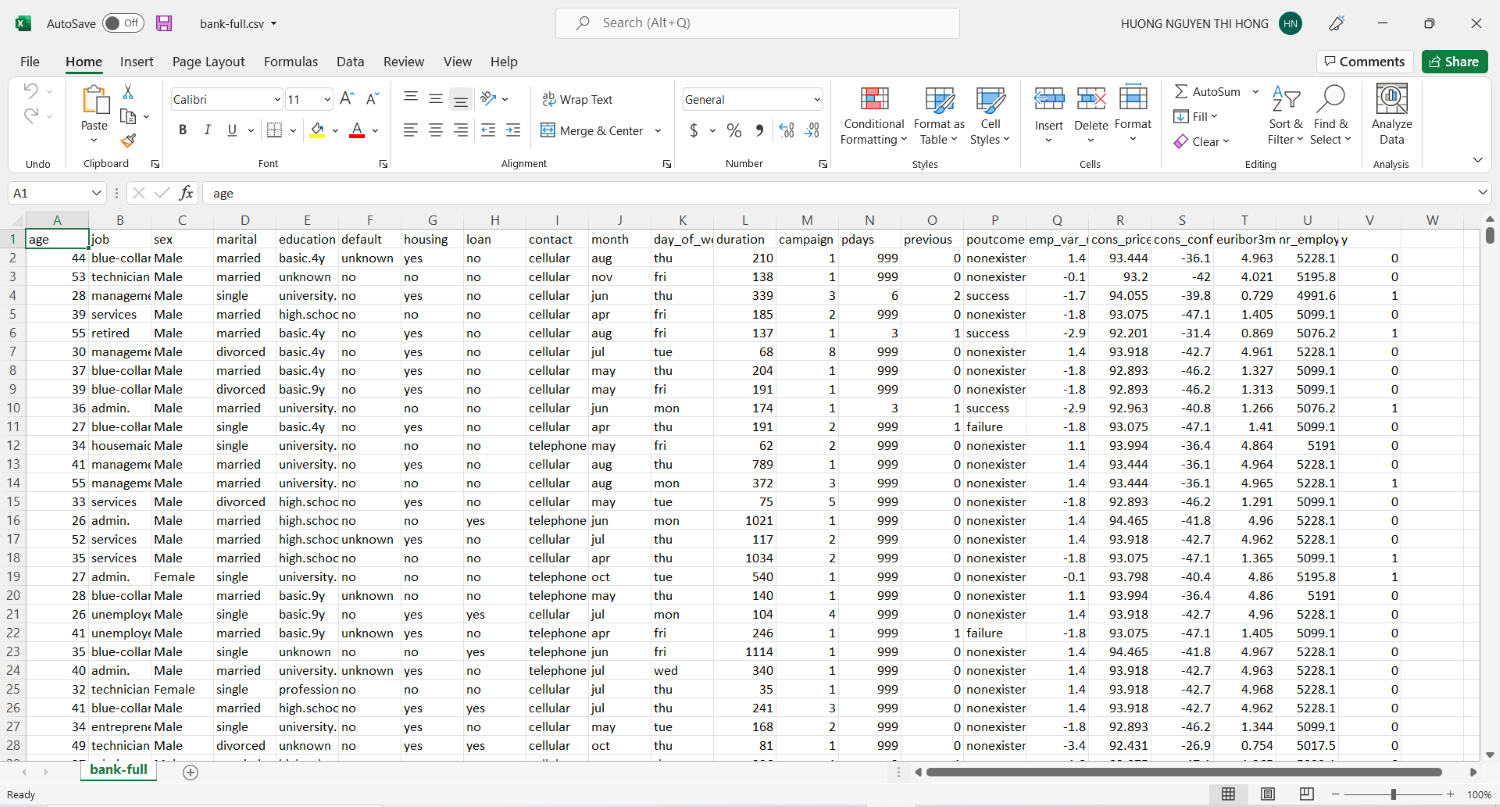
\includegraphics[scale = 0.5]{images/dataset.png}
    	\end{center}
    		\caption{Tập dữ liệu \textit{bank-full.csv}}
    \end{figure}
    \end{center}
\fontsize{14}{10}\selectfont
\section{Đặc tả tập dữ liệu}
     \fontsize{13}{14}\selectfont
      \begin{enumerate}
        \item age: số tuổi của khách hàng (kiểu dữ liệu số - numeric)
        \item job: loại công việc (phân loại:"admin.","blue-collar", "entrepreneur", "housemaid", "management", "retired", "self-employed", "services", "student", "technician", "unemployed", "unknown").
        \item sex: giới tính của khách hàng (phân loại: "Male", "Female").
        \item marital: tình trạng hôn nhân của khách hàng (phân loại: "divorced", "married", "single", "unknown").
        \item education: trình độ giáo dục (phân loại: "basic.4y", "basic.6y", "basic.9y", "high.school", "illiterate", "professional.course", "university.degree", "unknown").
        \item default: có tín dụng trong tình trạng vỡ nợ? (phân loại: "yes",  "no" và "unknown").
        \item housing: có cho vay mua nhà không? (phân loại: "yes",  "no" và "unknown").
        \item loan: có vay cá nhân không? (phân loại: "yes",  "no" và "unknown").
        \item contact: kiểu liên lạc (phân loại: "cellular", "telephone").
        \item month: tháng liên hệ cuối cùng trong năm (phân loại: “jan”, “feb”, “mar”,.., “nov”, “dec”).
        \item day\_of\_week: ngày liên hệ cuối cùng trong tuần (phân loại: “mon”, “tue”, “wed”, “thu”, “fri”).
        \item duration: thời lượng liên hệ cuối cùng, tính bằng giây (số). Lưu ý quan trọng: thuộc tính này ảnh hưởng nhiều đến mục tiêu đầu ra (ví dụ: nếu thời lượng = 0 thì y = ’không’). Khoảng thời gian không được biết trước khi cuộc gọi được thực hiện, cũng như sau khi kết thúc cuộc gọi, y hiển nhiên được biết. Do đó, đầu vào này chỉ nên được đưa vào cho các mục đích chuẩn và nên bị loại bỏ nếu mục đích là có một mô hình dự đoán thực tế.
        \item campaign: số liên hệ được thực hiện trong chiến dịch này và cho khách hàng này (kiểu số - numeric, bao gồm liên hệ cuối cùng)
        \item pdays: số ngày trôi qua sau khi khách hàng được liên hệ lần cuối từ một chiến dịch trước đó (kiểu dữ liệu số - numeric; 999 nghĩa là khách hàng không có sự tương tác trước đó)
        \item previous: số lượng địa chỉ liên hệ của khách hàng được thực hiện trước khi thực hiện việc thu thập dữ liệu (kiểu dữ liệu số - numeric)
        \item poutcome: : kết quả của chiến dịch tiếp thị trước đó (phân loại:“failure”, “nonexistent”, “success”")
        \item emp.var.rate: tỷ lệ biến động việc làm - chỉ số hàng quý (kiểu dữ liệu số - numeric)
        \item cons.price.idx: chỉ số giá tiêu dùng - chỉ số hàng tháng (kiểu dữ liệu số - numeric)     
        \item cons.conf.idx:  chỉ số niềm tin của khách hàng - chỉ số hàng tháng (kiểu dữ liệu - numeric)     
        \item euribor3m: euribor lãi suất 3 tháng - (kiểu dữ liệu số - numeric)
        \item nr.employed: số lượng nhân viên - chỉ số hàng quý (kiểu dữ liệu số - numeric)
        \item y - khách hàng đã đăng ký tiền gửi có kỳ hạn chưa? (nhị phân: "0" và "1")
    \end{enumerate}

\fontsize{14}{10}\selectfont
\section{Trực quan hóa bằng đồ thị}
\subsection{\textit{Số lượng khách hàng đăng ký một khoản tiền gửi có kỳ hạn}}

          \begin{center}
        \begin{figure}[htp]
    	\begin{center}
    		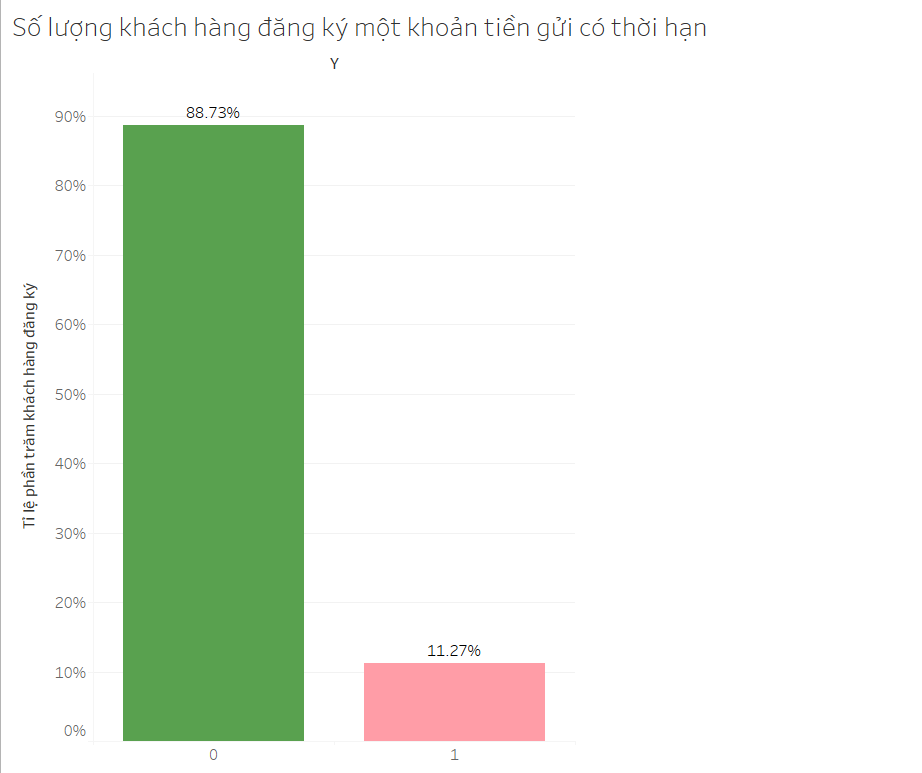
\includegraphics[width=11cm]{images/hinh1.png}
    	\end{center}
    		\caption{Đồ thị biểu diễn tỉ lệ khách hàng đăng ký gửi một khoản tiền có kỳ hạn}
    \end{figure}
    \end{center}
\fontsize{13}{14}\selectfont \textbf{$\star$\textit{ Nhận xét}}
    \begin{enumerate}
        \item [- ] Số lượng khách hàng không đăng ký chiếm đa số gần 90 phần trăm, trong khi đó khách hàng có đăng ký chỉ chiếm hơn 11 phần trăm.
        \item[- ] Dữ liệu bị nghiêng về một phía với tỉ lệ 9:1.
        \item [- ] Tập dữ liệu trên không cân bằng (Imbalanced data): mất cân bằng dữ liệu rất phổ biến trong các bài toán phân loại. Việc triển khai một cách cố gắng mô hình phân loại trên dữ liệu không cân bằng như vậy có thể sẽ dẫn đến độ chính xác dự đoán rất thấp. Trong khi đó, tỉ lệ trong bài toán trên lệch hẳn 9:1, cần phải có giải pháp để cải thiện cho mô hình trên bởi vì nếu có đưa ra dự đoán thì kết quả sẽ thiên về phía có phần trăm nhiều hơn dẫn đến dự đoán kém bên phía ít hơn.
    \end{enumerate}
    
\subsection{\textit{Số lượng khách hàng đăng ký theo nghề nghiệp}}
         \begin{center}
        \begin{figure}[htp]
    	\begin{center}
    		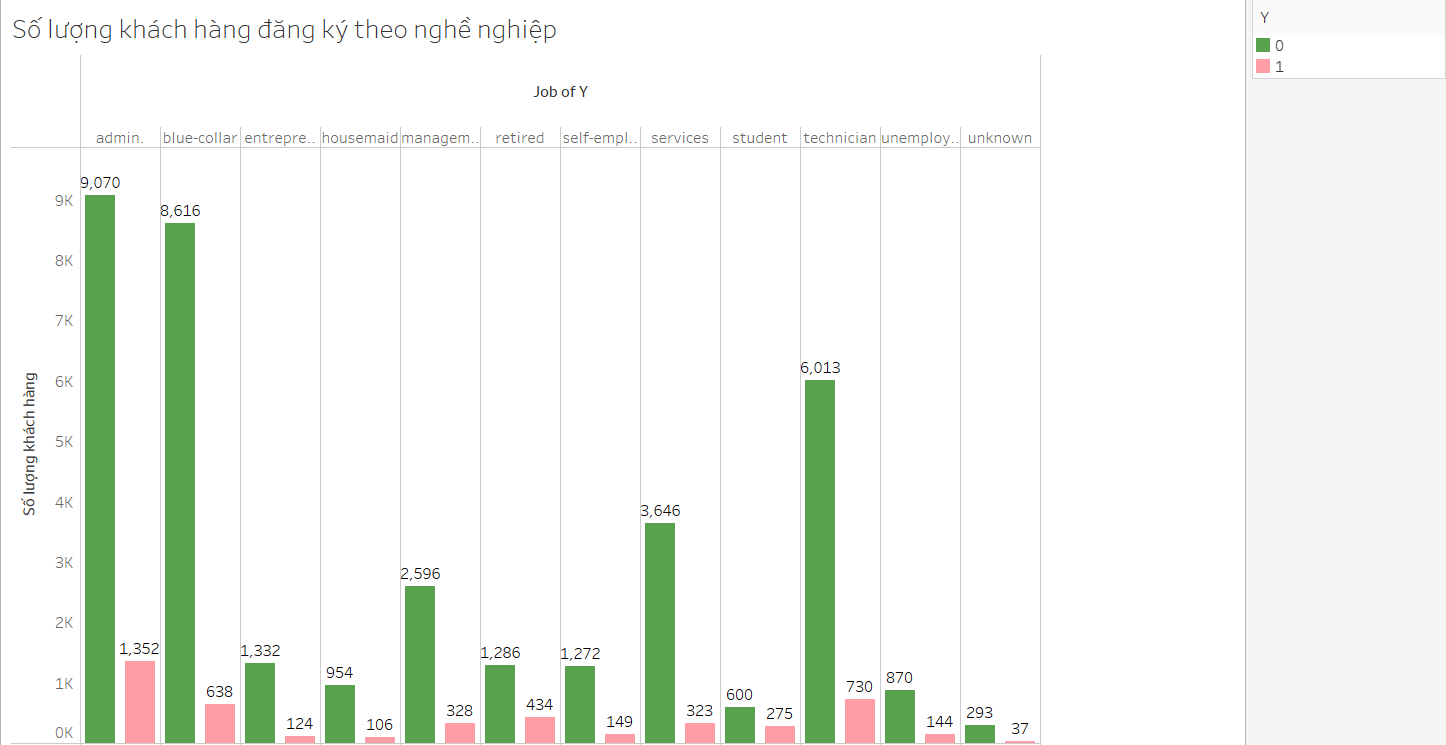
\includegraphics[width=15cm, height=9cm]{images/hinh2.png}
    	\end{center}
    		\caption{Đồ thị biểu diễn số lượng khách hàng đăng ký theo nghề nghiệp}
    \end{figure}
    \end{center}
    \fontsize{13}{14}\selectfont \textbf{$\star$\textit{ Nhận xét}}
    \begin{enumerate}
        \item[- ] Đồ thị biểu diễn số khách hàng đăng ký thông qua các nghề nghiệp là khác nhau và không đồng đều.
        \item[- ] Admin chiếm giá trị cao nhất trong trường hợp về số người không đăng ký và có đăng ký.
        \item[- ] Unknown chiếm giá trị thấp nhất trong trường hợp về số người đăng ký và không đăng ký.
        \item[- ]'Job' là một biến độc lập (Independent variable) mang các yếu tố hay điều kiện mà khi thay đổi sẽ ảnh hưởng đến kết quả dự đoán cho y (outcome variable). Đây là biến mang nhiều yếu tố dự đoán cho biến y (kết quả dự đoán của biến y sẽ thay đổi ít nhiều theo biến độc lập).
    \end{enumerate}
    
\subsection{\textit{Số lượng khách hàng đăng ký theo tình trạng hôn nhân}}
         \begin{center}
        \begin{figure}[htp]
    	\begin{center}
    		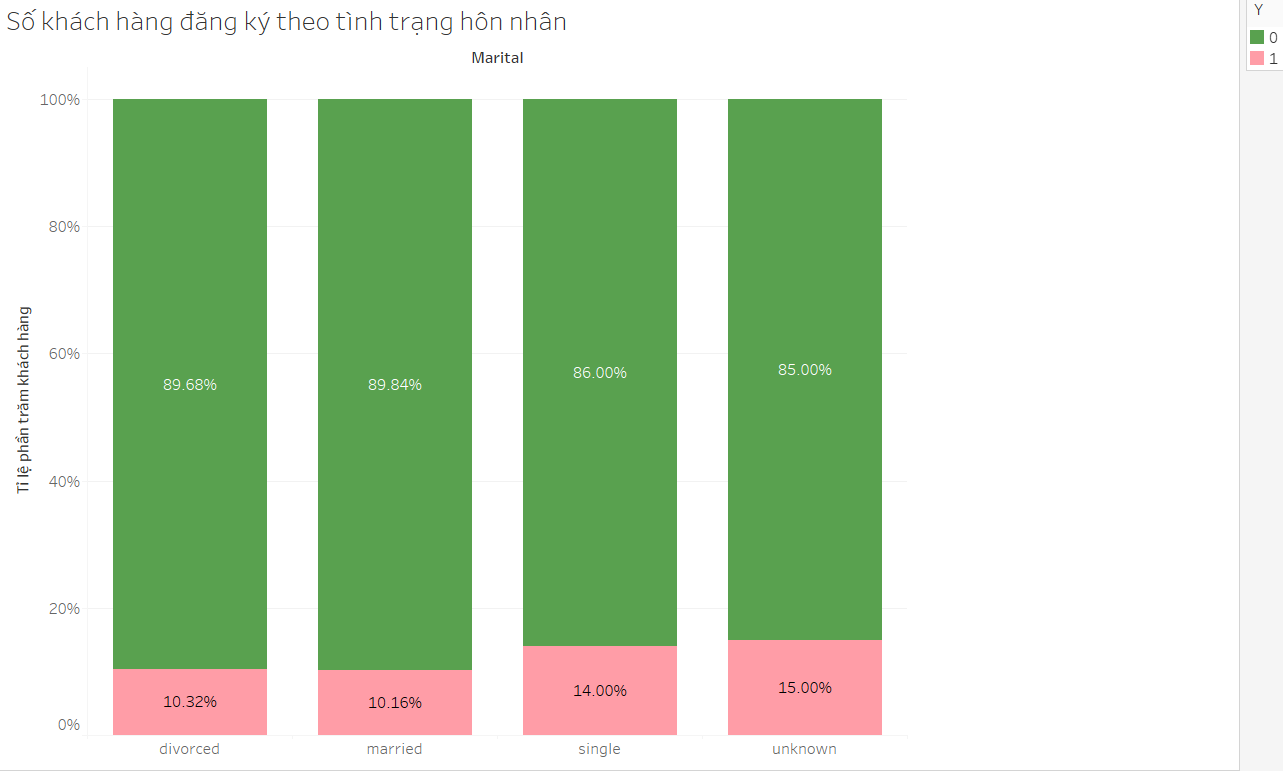
\includegraphics[width=15cm, height=9cm]{images/hinh3.png}
    	\end{center}
    		\caption{Đồ thị biểu diễn số phần trăm khách hàng đăng ký theo tình trạng hôn nhân}
    \end{figure}
    \end{center}
    \fontsize{13}{14}\selectfont \textbf{$\star$\textit{ Nhận xét}}
    \begin{enumerate}
        \item[- ] Single và Unknown có tỉ lệ gần như bằng nhau trong trường hợp khách hàng không đăng ký và có đăng ký, chỉ hơn kém 1\%.
        \item[- ] Divorced và married: cũng tương tự như trường hợp trên về cả khách hàng đăng ký hay không đăng ký.
        \item[- ] Các tỉ lệ theo tình trạng hôn nhân không chênh lệch nhiều.
        \item [$\Rightarrow$] Ta thấy biến độc lập marital không phải là yếu tố dự đoán tốt cho biến outcome y.
    \end{enumerate}

\subsection{\textit{Số lượng khách hàng đăng ký theo trình độ giáo dục}}
         \begin{center}
        \begin{figure}[htp]
    	\begin{center}
    		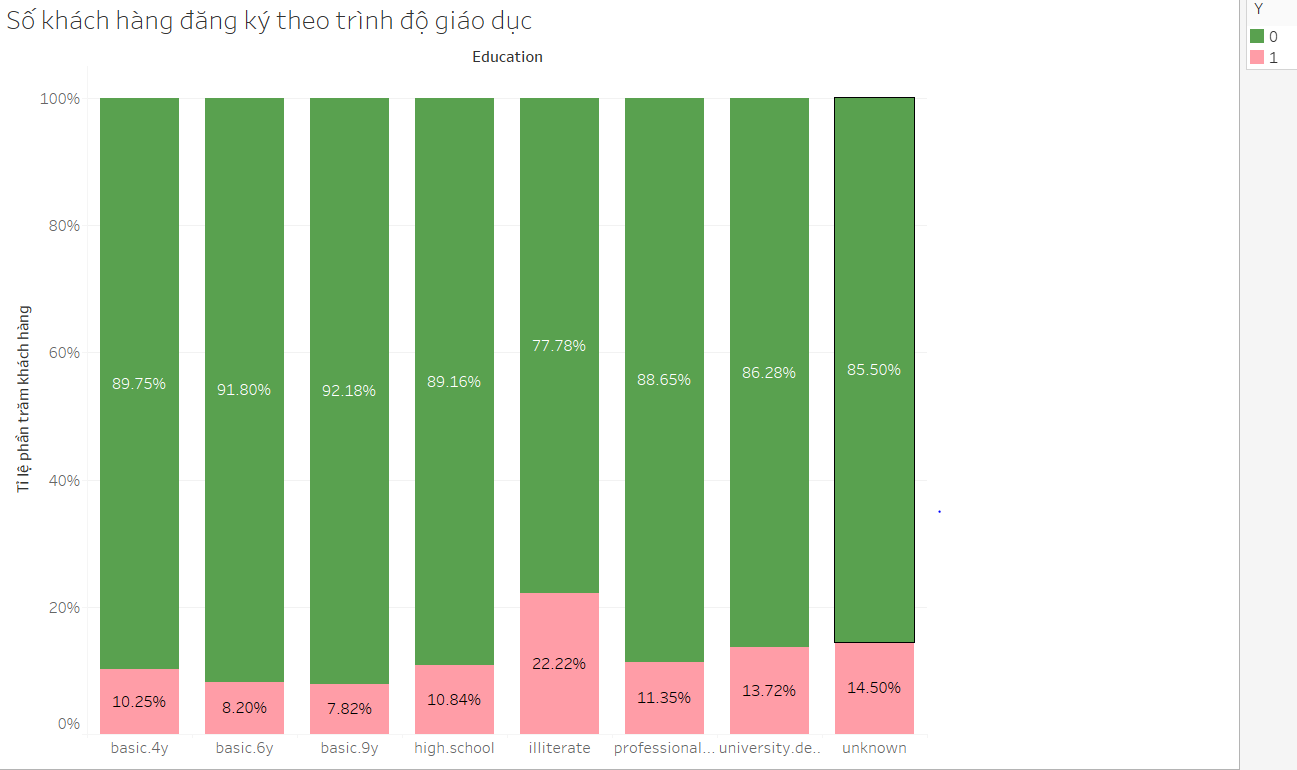
\includegraphics[width=15cm, height=9cm]{images/hinh4.png}
    	\end{center}
    		\caption{Đồ thị biểu diễn số phần trăm khách hàng đăng ký theo trình độ giáo dục}
    \end{figure}
    \end{center}
    \fontsize{13}{14}\selectfont \textbf{$\star$\textit{ Nhận xét}}
    \begin{enumerate}
        \item[- ] Illiterate có phần trăm số khách hàng đăng ký nhiều nhất và phần trăm khách hàng không đăng ký là thấp nhất.
        \item[- ] Cột basic.4y, basic.6y, basic.9y có số phần trăm khách hàng không đăng ký cao nhất và khách hàng đăng ký thấp nhất.
        \item [$\Rightarrow$] Ta thấy biến độc lập education là yếu tố dự đoán tốt cho biến outcome y.
    \end{enumerate}
\pagebreak
\subsection{\textit{Số lượng khách hàng đăng ký theo ngày}}
         \begin{center}
        \begin{figure}[htp]
    	\begin{center}
    		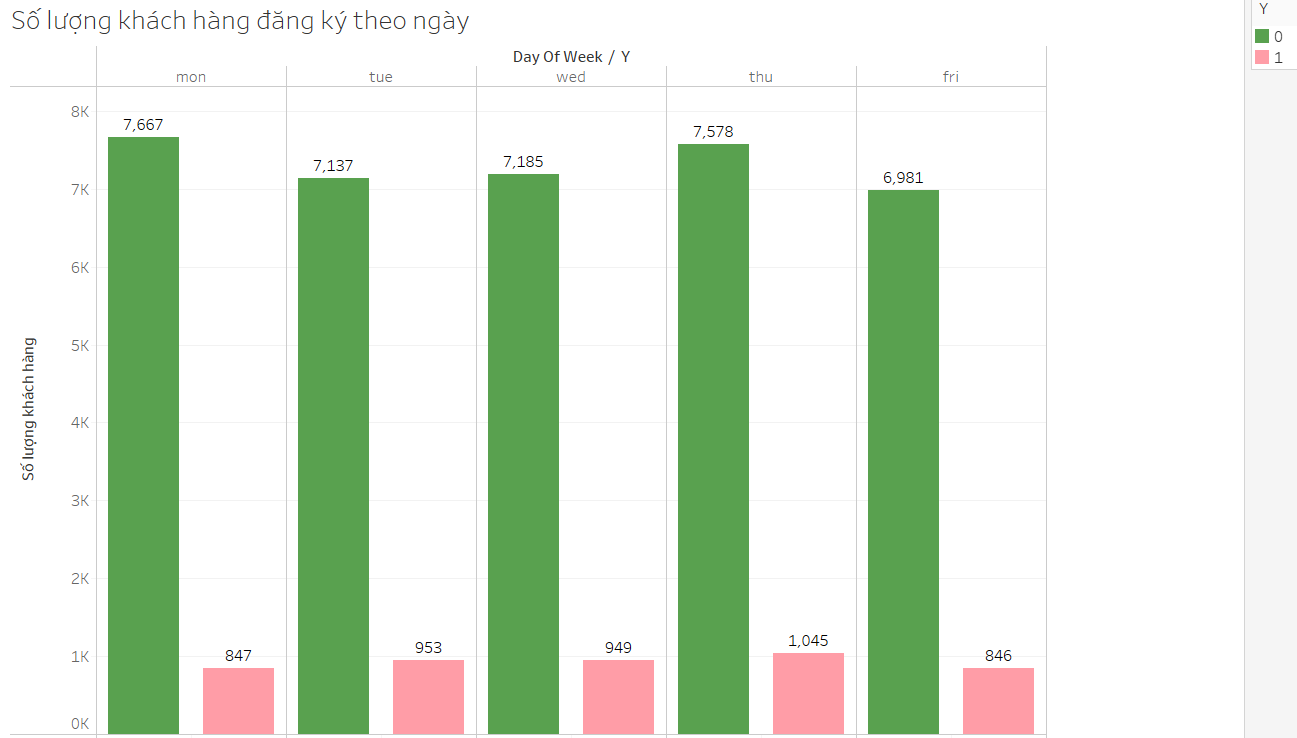
\includegraphics[width=15cm, height=9cm]{images/hinh5.png}
    	\end{center}
    		\caption{Đồ thị biểu diễn số lượng khách hàng đăng ký theo ngày trong tuần}
    \end{figure}
    \end{center}
    \fontsize{13}{14}\selectfont \textbf{$\star$\textit{ Nhận xét}}
    \begin{enumerate}
        \item[- ] Số lượng khách hàng đăng ký vào các ngày trong tuần cũng không chênh lệch quá nhiều giữa các ngày với nhau.
        \item[- ] Dữ liệu bị nghiêng về phía khách hàng không đăng ký.
        \item [$\Rightarrow$] Ta thấy biến độc lập dayofweek không là yếu tố dự đoán tốt cho biến outcome y.
    \end{enumerate}
\pagebreak

\subsection{\textit{Số lượng khách hàng đăng ký theo tháng}}
         \begin{center}
        \begin{figure}[htp]
    	\begin{center}
    		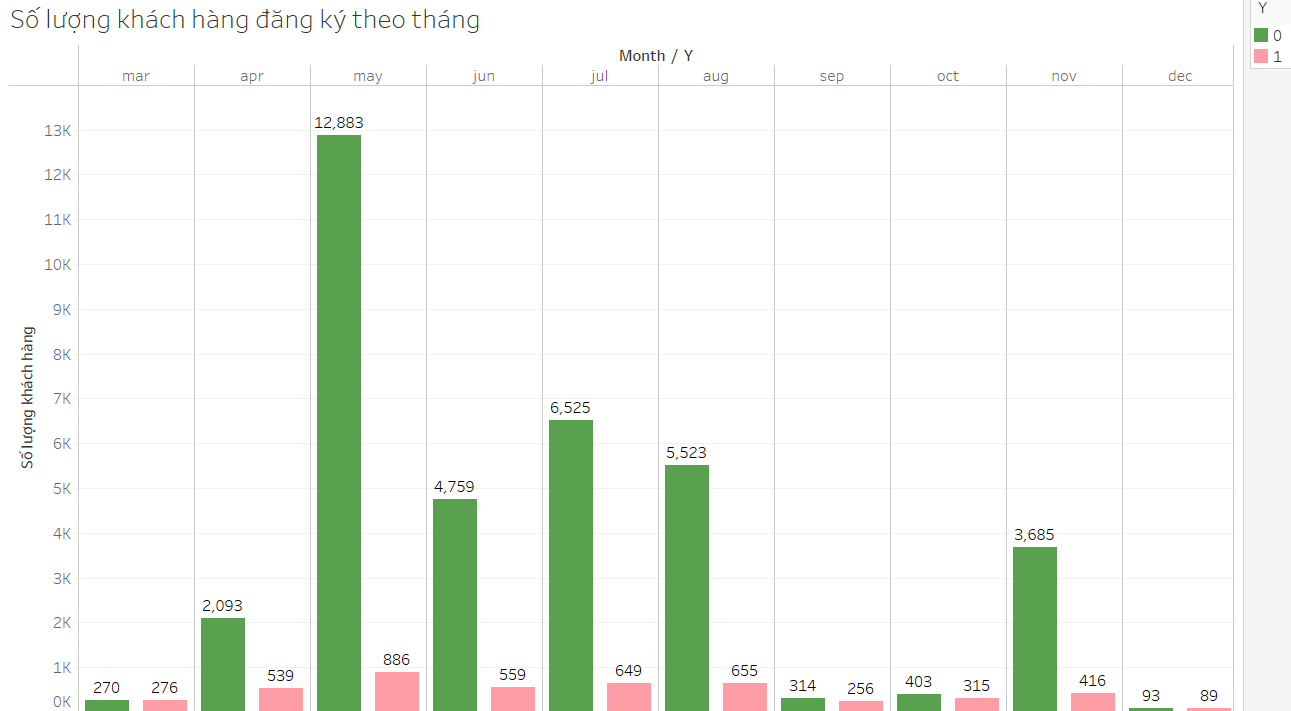
\includegraphics[width=15cm, height=9cm]{images/hinh6.png}
    	\end{center}
    		\caption{Đồ thị biểu diễn số lượng khách hàng đăng ký theo tháng}
    \end{figure}
    \end{center}
    \fontsize{13}{14}\selectfont \textbf{$\star$\textit{ Nhận xét}}
    \begin{enumerate}
        \item[- ] May có số khách hàng không đăng ký nhiều nhất và số người đăng ký cao nhất.
        \item[- ] Dec thì ngược lại, không đăng ký và có đăng ký đều ít nhất.
        \item[- ] Số lượng biến động khách hàng theo tháng có sự thay đổi không đồng đều.
        \item [$\Rightarrow$] Ta thấy biến độc lập month là yếu tố dự đoán tốt cho biến outcome y.
    \end{enumerate}
\pagebreak

\subsection{\textit{Số lượng khách hàng đăng ký theo tình trạng tiếp thị trước đó}}
         \begin{center}
        \begin{figure}[htp]
    	\begin{center}
    		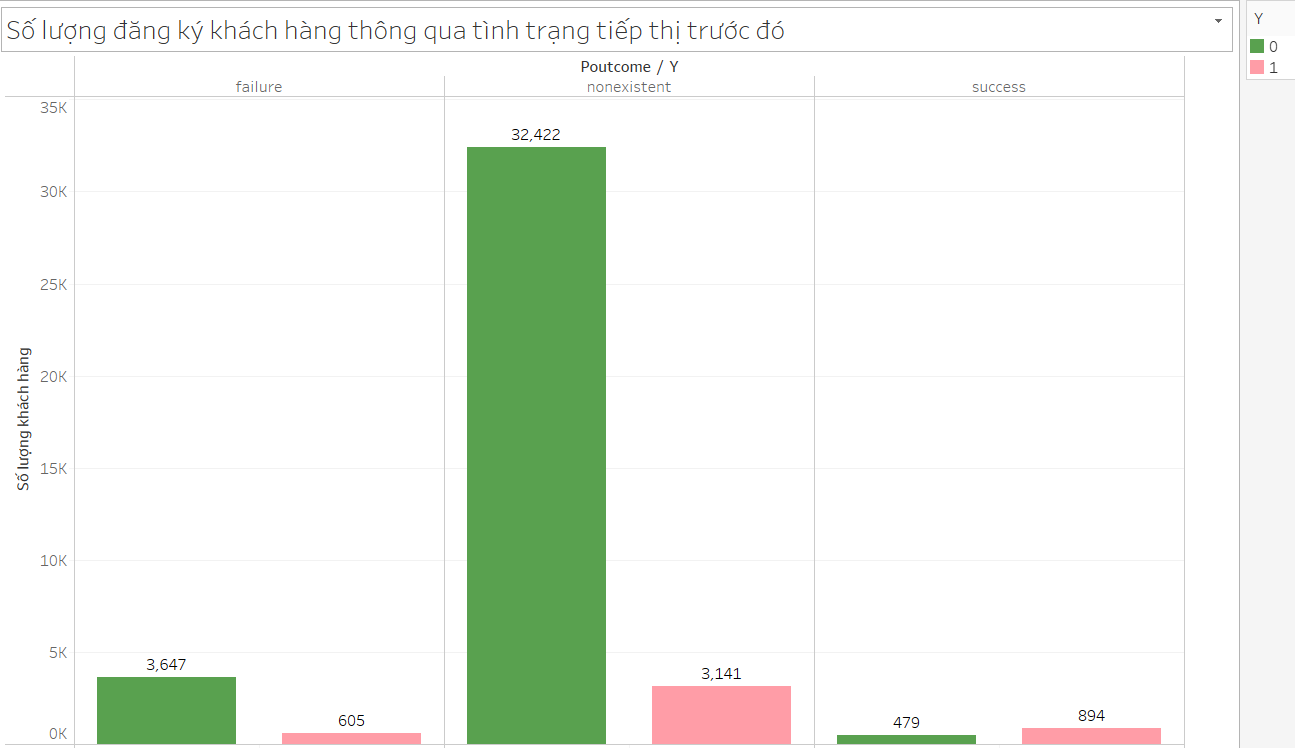
\includegraphics[width=15cm, height=9cm]{images/hinh7.png}
    	\end{center}
    		\caption{Đồ thị biểu diễn số lượng khách hàng đăng ký theo tình trạng tiếp thị trước đó}
    \end{figure}
    \end{center}
    \fontsize{13}{14}\selectfont \textbf{$\star$\textit{ Nhận xét}}
    \begin{enumerate}
        \item[- ] Nonexistent có số khách hàng không ký và đăng ký chiếm cao nhất. 
        \item[- ] Success thì có số khách hàng không đăng ký và đăng ký chiếm thấp nhất.
        \item[- ] Cả 3 tình trạng nhìn chung có sự chênh lệch với nhau.
        \item [$\Rightarrow$] Ta thấy biến độc lập poutcome là yếu tố dự đoán tốt cho biến outcome y.
    \end{enumerate}
\pagebreak
\subsection{\textit{Số lượng khách hàng đăng ký theo giới tính}}
         \begin{center}
        \begin{figure}[htp]
    	\begin{center}
    		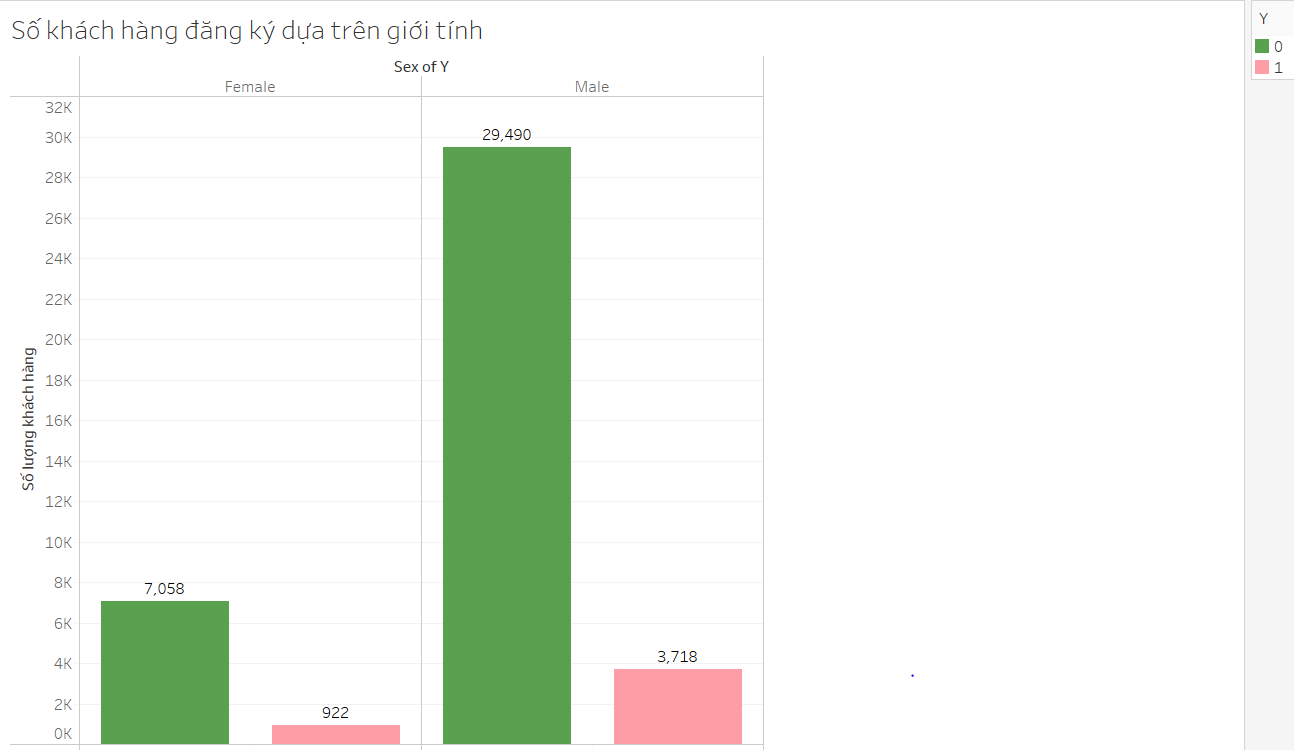
\includegraphics[width=15cm, height=9cm]{images/hinh9.png}
    	\end{center}
    		\caption{Đồ thị biểu diễn số lượng khách hàng đăng ký theo giới tính}
    \end{figure}
    \end{center}
    \fontsize{13}{14}\selectfont \textbf{$\star$\textit{ Nhận xét}}
    \begin{enumerate}
        \item[- ] Dịch vụ tiếp thị có khách hàng là nam chiếm đa số.
        \item[- ] Giới tính có ảnh hưởng rất nhiều đến chiến dịch tiếp thị trực tiếp này.
        \item [$\Rightarrow$] Ta thấy biến độc lập sex là yếu tố dự đoán tốt cho biến outcome y.
    \end{enumerate}
\pagebreak
\subsection{\textit{Số lượng khách hàng theo độ tuổi}}
         \begin{center}
        \begin{figure}[htp]
    	\begin{center}
    		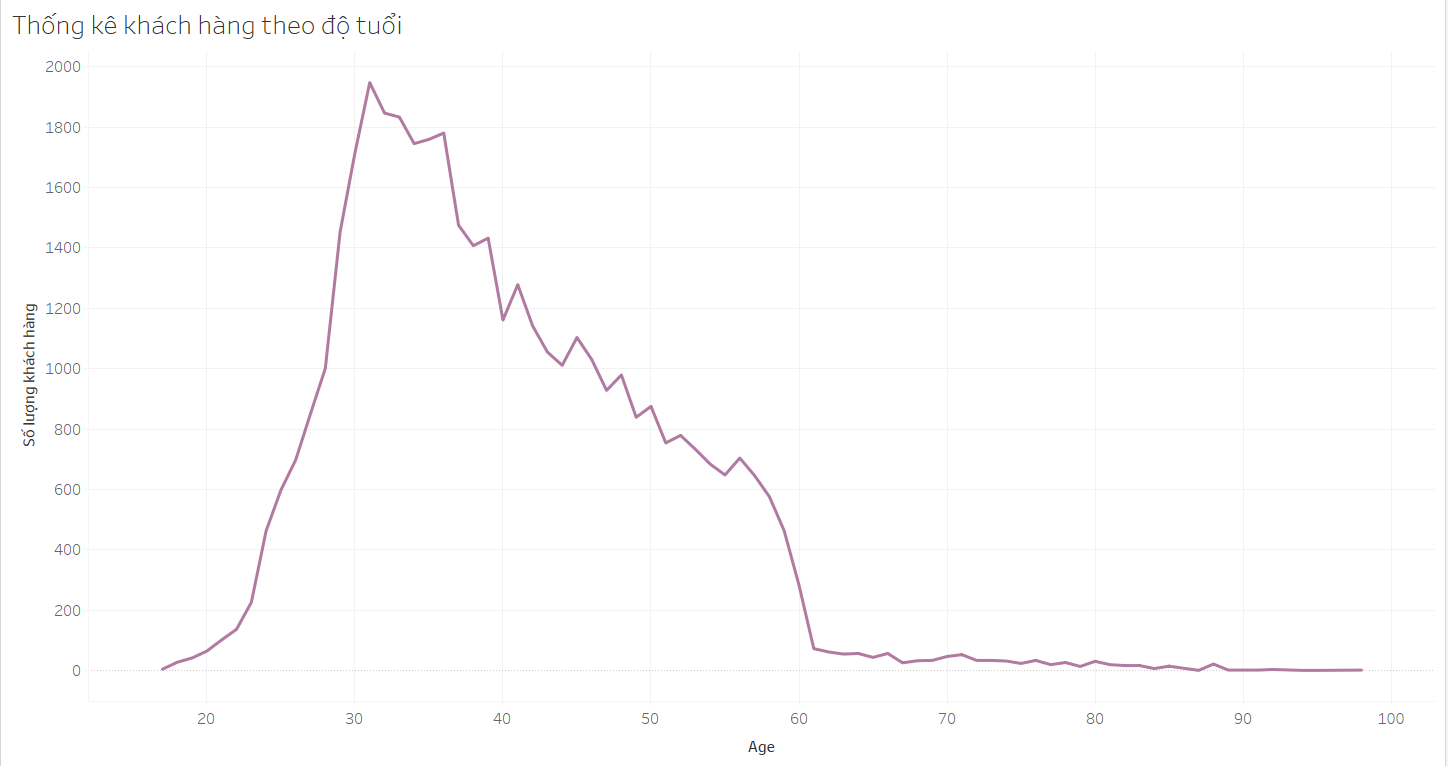
\includegraphics[width=15cm, height=9cm]{images/hinh8.png}
    	\end{center}
    		\caption{Đồ thị biểu diễn số lượng khách hàng theo độ tuổi}
    \end{figure}
    \end{center}
    \fontsize{13}{14}\selectfont \textbf{$\star$\textit{ Nhận xét}}
    \begin{enumerate}
        \item[- ] Hầu hết các khách hàng đến với dịch vụ nằm trong khoảng từ 30 đến 50 tuổi. 
        \item[- ] Độ tuổi của khách hàng có ảnh hưởng rất lớn đối với chiến dịch tiếp thị trực tiếp này.
        \item [$\Rightarrow$] Ta thấy biến độc lập age là yếu tố dự đoán tốt cho biến outcome y.
    \end{enumerate}
   \fontsize{13}{14}\selectfont\textbf{\underline{\underline{{KẾT LUẬN}}}}:
   \begin{enumerate}
        \item [- ] Trong tập dữ liệu, các biến độc lập khác nhau mang ảnh hưởng, tác động khác nhau trong việc dự đoán biến y. 
        \item [- ] Tập dữ liệu bị mất cân bằng có thể đề ra giải pháp để cân bằng nhằm dự đoán chính xác hơn và cũng nhằm so sánh giữa tập dữ liệu đã cân bằng với tập dữ liệu gốc.
    \end{enumerate}
\fontsize{14}{10}\selectfont
\section{Xử lý tập dữ liệu}
 \subsection{ \textit{Quá trình xử lí dữ liệu}}
        \fontsize{13}{14}\selectfont
        \begin{enumerate}
                    \item [- ] Đơn giản hóa dữ liệu: Ở biến độc lập \textit{education}, thực hiện việc gôm nhóm các dữ liệu \textit{basic.4y}, \textit{basic.6y} và \textit{basic.9y} thành \textit{basic}.
                     \begin{center}
        \begin{figure}[htp]
    	\begin{center}
    		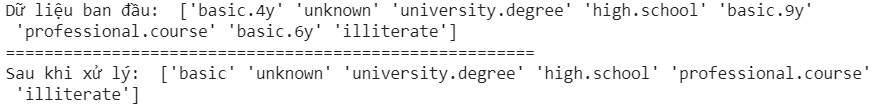
\includegraphics[scale =0.7]{images/basic.png}
    	\end{center}
    		\caption{Dữ liệu trước và sau khi xử lý ở cột education}
    \end{figure}
        \end{center}
    \item [- ]	Tạo biến giả (Dummy variable):
                        \begin{itemize}
                            \item Biến giả là biến độc lập được đưa vào mô hình hồi qui để giải thích các yếu tố định tính.
                            \item Chuyển đổi biến độc lập loại chuỗi thành các biến độc lập loại số dạng nhị phân (1 hoặc 0).
                            \item [$\diamond$] Ví dụ: Từ biến độc lập marital ta khởi tạo thành một biến giả dạng nhị phân 
                            \newline\tab[1.25cm] marital = married
                            \newline\tab[1.25cm] marital-married = 1 nếu khách hàng đó có kết hôn
                            \newline\tab[1.25cm] marital-married = 0 nếu khách hàng không có kết hôn
                        \end{itemize}
                        
                    \item [- ] Các biến độc lập cần xử lý dữ liệu:
                        \begin{itemize}
                        \item Sex:
                                \newline\tab “Male”, “Female"
                            \item Job:
                                \newline\tab “admin”, “blue-collar”, “entrepreneur”, “housemaid”,
                                \newline\tab “management”, “retired”, “self-employed”, “services”,
                                \newline\tab “student”, “technician”, “unemployed”, “unknown”
                            \item marital:
                                \newline\tab “divorced”, “married”, “single”, “unknown”
                            \item education:
                                \newline\tab “basic”, “high.school”, “illiterate”, “professional.course”, 
                                \newline\tab “university.degree”, “unknown”
                            \item default:
                                \newline\tab “no”, “yes”, “unknown”
                                
                            \item housing:
                                \newline\tab “no”, “yes”, “unknown”
                            \item loan:
                                \newline\tab “no”, “yes”, “unknown”
                            \item contact:
                                \newline\tab “cellular”, “telephone”
                            \item month:
                                \newline\tab “jan”, “feb”, “mar”,..., “nov”, “dec”
                            \item day\_of\_week:
                                \newline\tab “mon”, “tue”, “wed”, “thu”, “fri”
                            \item poutcome:
                                \newline\tab “failure”, “nonexistent”, “success”
                        \end{itemize}
    \begin{center}
        \begin{figure}[htp]
    	\begin{center}
    		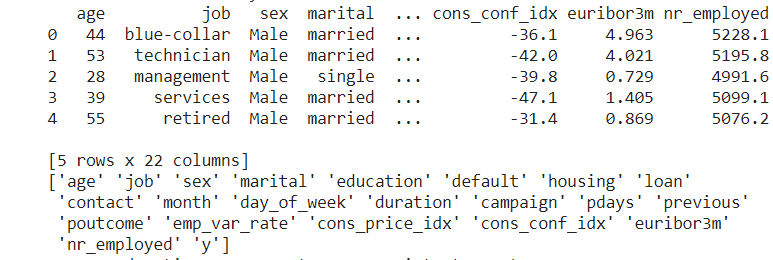
\includegraphics[scale =0.9]{images/nummy1.PNG}
    	\end{center}
    		\caption{Dữ liệu trước khi tạo biến giả}
    \end{figure}
        \end{center}
\pagebreak
            \begin{center}
        \begin{figure}[htp]
    	\begin{center}
    		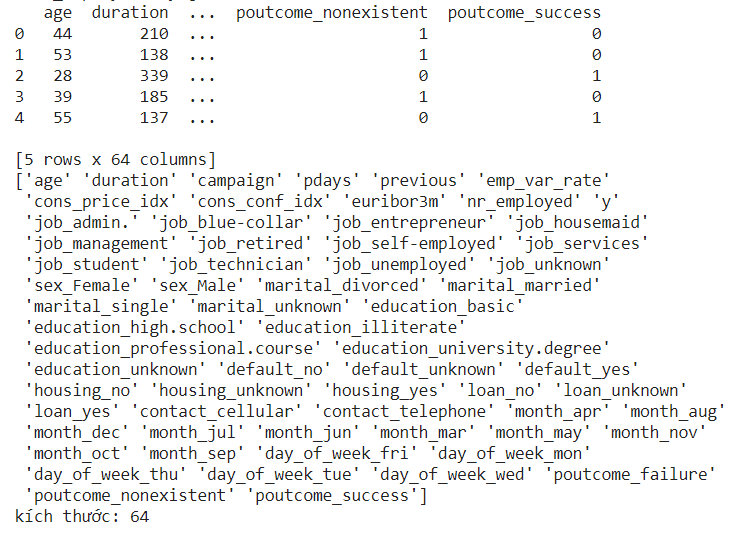
\includegraphics[scale =0.9]{images/nummy2.PNG}
    	\end{center}
    		\caption{Dữ liệu sau khi tạo biến giả}
    \end{figure}
        \end{center}
        \end{enumerate}
 \subsection{ \textit{Phương pháp SMOTE}}
        \fontsize{13}{14}\selectfont
    \begin{itemize}
                        \item [- ]Tạo dữ liệu mẫu giả cho tập thiểu số sao cho số phần tử của nó được nhiều lên bằng cách là lặp lại mỗi điểm trong nhóm thiểu số nhiều lần.
                        \item [- ]SMOTE (Synthetic Minority Over-sampling): là phương pháp sinh mẫu nhằm gia tăng kích thước mẫu của nhóm thiểu số trong trường hợp xảy ra mất cân bằng mẫu. Để gia tăng kích thước mẫu, với mỗi một mẫu thuộc nhóm thiểu số sẽ lựa chọn ra k mẫu láng giềng gần nhất với nó và sau đó thực hiện tổ hợp tuyến tính để tạo ra mẫu giả lập.
\end{itemize}
\pagebreak
            \begin{center}
        \begin{figure}[htp]
    	\begin{center}
    		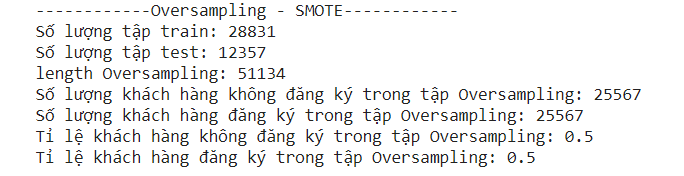
\includegraphics[scale =1]{images/smote.PNG}
    	\end{center}
    		\caption{Dữ liệu sau khi dùng SMOTE}
    \end{figure}
        \end{center}
  
  %-------------------------------------------------------------------------------------------------------------
%---------------Chương 4 -----------------------
\fontsize{16}{10}\selectfont
\chapter{THỰC NGHIỆM}
\fontsize{14}{10}\selectfont
\section{Thuật toán KNN}
     \fontsize{13}{14}\selectfont
     \begin{enumerate}
    \item [- ]	Tập dữ liệu gốc:
    \begin{center}
        \begin{figure}[htp]
    	\begin{center}
    		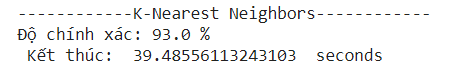
\includegraphics[scale =1.5]{images/knn_o.PNG}
    	\end{center}
    		\caption{Kết quả sau khi áp dụng thuật toán}
    \end{figure}
        \end{center}
\pagebreak
       \begin{center}
        \begin{figure}[htp]
    	\begin{center}
    		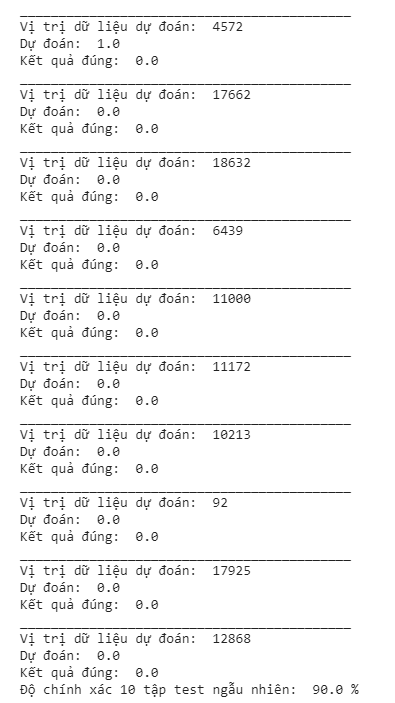
\includegraphics[scale =0.8]{images/knn_10_o.PNG}
    	\end{center}
    		\caption{Kết quả dự đoán 10 tập ngẫu nhiên}
    \end{figure}
        \end{center}    
        \item [- ]	Tập dữ liệu đã được cân bằng: chia dữ liệu thành hai tập train, tỉ lệ 7:3.
         \begin{center}
        \begin{figure}[htp]
    	\begin{center}
    		
\includegraphics[scale =1]{images/knn_smo.PNG}
    	\end{center}
    		\caption{Kết quả sau khi áp dụng thuật toán với dữ liệu cân bằng}
    \end{figure}
        \end{center}
\pagebreak
     \begin{center}
        \begin{figure}[htp]
    	\begin{center}
    		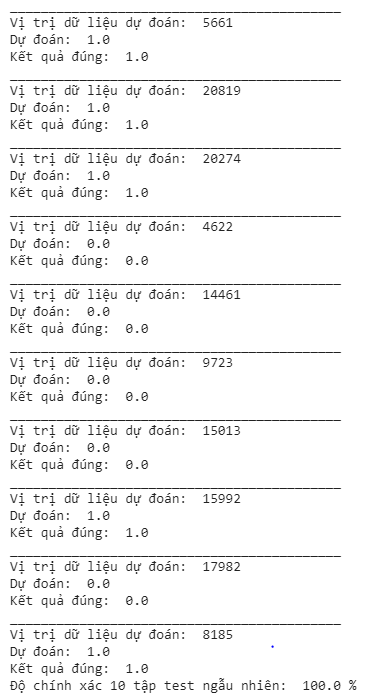
\includegraphics[scale =0.8]{images/knn_10_smo.PNG}
    	\end{center}
    		\caption{Kết quả dự đoán 10 tập ngẫu nhiên}
    \end{figure}
        \end{center} 
    \item [- ]	Nhận xét:
     \begin{itemize}
            \item Dữ liệu gốc khi tiến hành thực thi thuật toán lại có độ chính xác cao hơn đối với tập cân bằng với phương pháp SMOTE.
            \item Khi chọn K ta cần phải lưu ý vào tập dữ liệu và số lượng dữ liệu vì nếu chọn K quá nhỏ thì dữ liệu dự đoán sẽ bị nhiều.
            \item Kết quả dự đoán 10 tập ngẫu nhiên ở dữ liệu đã cân bằng lại mang chính xác 100\% với dữ liệu gốc chỉ 90\%
    \end{itemize}
    \end{enumerate}
\section{Thuật toán hồi quy logistic}
     \fontsize{13}{14}\selectfont
     \begin{enumerate}
    \item [- ]	Tập dữ liệu gốc:
\pagebreak
         \begin{center}
        \begin{figure}[htp]
    	\begin{center}
    		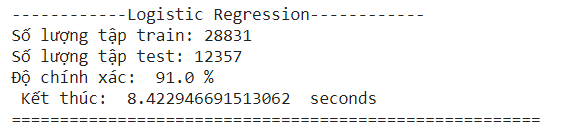
\includegraphics[scale =0.8]{images/lr_o.PNG}
    	\end{center}
    		\caption{Kết quả sau khi áp dụng thuật toán}
    \end{figure}
        \end{center} 
                 \begin{center}
        \begin{figure}[htp]
    	\begin{center}
    		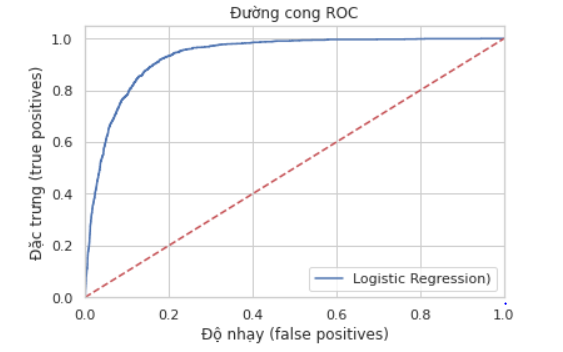
\includegraphics[scale =1]{images/lr_roc_o.PNG}
    	\end{center}
    		\caption{Đồ thị đường cong ROC}
    \end{figure}
        \end{center} 
    \item [- ]	Tập dữ liệu đã được cân bằng: chia dữ liệu thành hai tập train, tỉ lệ 7:3.
         \begin{center}
        \begin{figure}[htp]
    	\begin{center}
    		
\includegraphics[scale =01]{images/lr_smo.PNG}
    	\end{center}
    		\caption{Kết quả sau khi áp dụng thuật toán với dữ liệu cân bằng}
    \end{figure}
        \end{center}
\pagebreak
                 \begin{center}
        \begin{figure}[htp]
    	\begin{center}
    		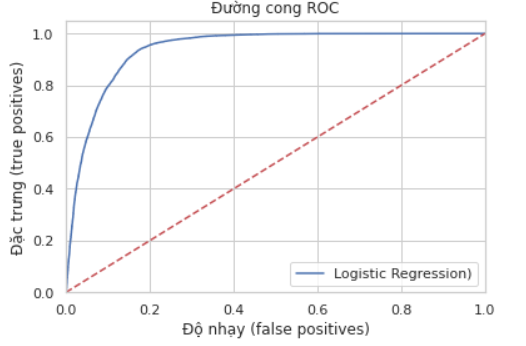
\includegraphics[scale =1]{images/lr_roc_smo.PNG}
    	\end{center}
    		\caption{Đồ thị đường cong ROC với dữ liệu cân bằng}
    \end{figure}
        \end{center} 
\item [- ]	Nhận xét:
     \begin{itemize}
            \item Dữ liệu khi tiến hành thực thi thuật toán ta thấy dữ liệu cân bằng với dữ liệu gốc có độ chính xác bằng nhau.
            \item Đường cong ROC dùng để đánh giá kết quả của một dự đoán, ta thấy đường cong của cả hai trường hợp đều có dấu hiệu đi lên dọc theo bìa trái chứng tỏ thuật toán áp dụng có độ chính xác rất tốt.
    \end{itemize}
    \end{enumerate}

\section{Thuật toán Naive Bayes}
     \fontsize{13}{14}\selectfont
     \begin{enumerate}
    \item [- ]	Tập dữ liệu gốc:
         \begin{center}
        \begin{figure}[htp]
    	\begin{center}
    		
\includegraphics[scale =1]{images/nb_o.PNG}
    	\end{center}
    		\caption{Kết quả sau khi áp dụng thuật toán}
    \end{figure}
        \end{center} 
    \item [- ]	Tập dữ liệu đã được cân bằng: chia dữ liệu thành hai tập train, tỉ lệ 7:3.
         \begin{center}
        \begin{figure}[htp]
    	\begin{center}
    		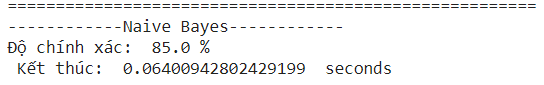
\includegraphics[scale =1]{images/nb_smo.PNG}
    	\end{center}
    		\caption{Kết quả sau khi áp dụng thuật toán với dữ liệu cân bằng}
    \end{figure}
        \end{center}
\item [- ]	Nhận xét:
     \begin{itemize}
            \item Dữ liệu khi tiến hành thực thi thuật toán ta thấy dữ liệu cân bằng với dữ liệu gốc có độ chính xác gần bằng nhau, hơn nhau chỉ 1 \%
            \item Độ chính xác của thuật toán cũng khá cao nhưng không cao bằng hai thuật toán trước đó.
    \end{itemize}
    \end{enumerate}
    
\section{Thuật toán Support Vector Machine}
     \fontsize{13}{14}\selectfont
     \begin{enumerate}
    \item [- ]	Tập dữ liệu gốc:
         \begin{center}
        \begin{figure}[htp]
    	\begin{center}
    		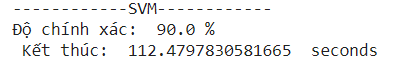
\includegraphics[scale =1]{images/svm_o.PNG}
    	\end{center}
    		\caption{Kết quả sau khi áp dụng thuật toán}
    \end{figure}
        \end{center} 
    \item [- ]	Tập dữ liệu đã được cân bằng: chia dữ liệu thành hai tập train, tỉ lệ 7:3.
         \begin{center}
        \begin{figure}[htp]
    	\begin{center}
    		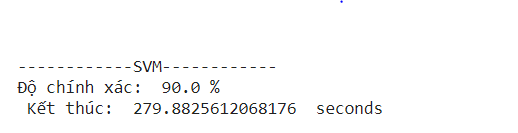
\includegraphics[scale =1]{images/svm_smo.PNG}
    	\end{center}
    		\caption{Kết quả sau khi áp dụng thuật toán với dữ liệu cân bằng}
    \end{figure}
        \end{center}
\item [- ]	Nhận xét:
     \begin{itemize}
            \item Dữ liệu khi tiến hành thực thi thuật toán ta thấy dữ liệu cân bằng với dữ liệu gốc có độ chính xác giống nhau.
            \item Độ chính xác của thuật toán cao, tuy nhiên thời gian thực thi lại chậm hơn rất nhiều so với các thuật toán trước đó.
    \end{itemize}
    \end{enumerate}
    
\section{Thuật toán Decision Tree}
     \fontsize{13}{14}\selectfont
     \begin{enumerate}
    \item [- ]	Tập dữ liệu gốc:
         \begin{center}
        \begin{figure}[htp]
    	\begin{center}
    		
\includegraphics[scale =1]{images/dt_o.PNG}
    	\end{center}
    		\caption{Kết quả sau khi áp dụng thuật toán}
    \end{figure}
        \end{center} 
         \begin{center}
        \begin{figure}[htp]
    	\begin{center}
    		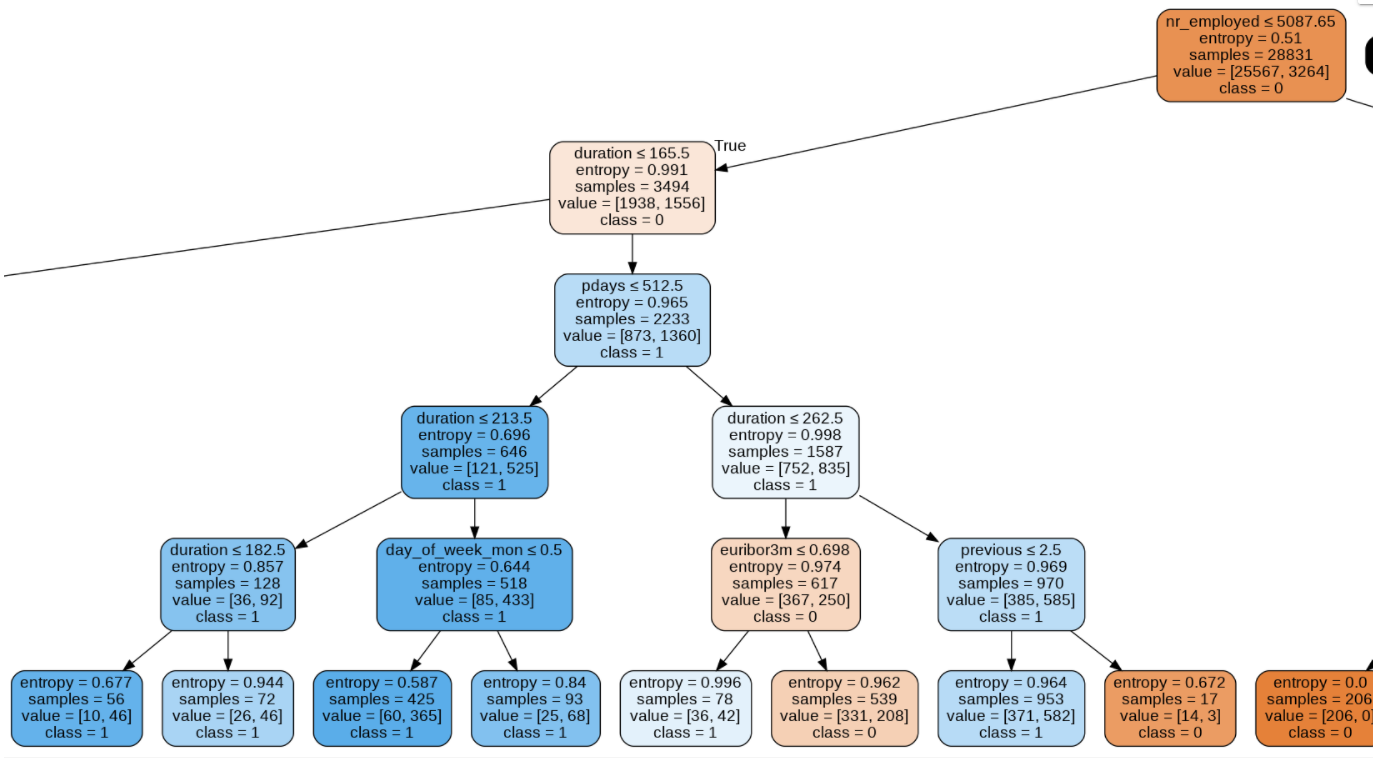
\includegraphics[scale =0.5]{images/tree_gra_o.PNG}
    	\end{center}
    		\caption{Hình ảnh một phần của cây quyết định với tập dữ liệu gốc}
    \end{figure}
        \end{center}
        \begin{itemize}
            \item Chọn thuộc tính nr\_employed làm gốc vì nó có giá trị Gain lớn nhất.
            \item samples ở đây chứa 28831 có nghĩa là cây này được training 28831 mẫu dữ liệu.
            \item Value [25567, 3264] là giá trị lớp mẫu, tức là có 25567 thuộc lớp 0, còn lại phân vào lớp 1. Lớp 0 có giá trị lớn hơn nên gốc cây này phân vào lớp 0.
            \item So sánh điều kiện với nr\_employed nếu đúng thì nó sẽ phân nhánh ra cây con mới bên trái.
    \end{itemize}
    \item [- ]	Tập dữ liệu đã được cân bằng: chia dữ liệu thành hai tập train, tỉ lệ 7:3.
         \begin{center}
        \begin{figure}[htp]
    	\begin{center}
    		
\includegraphics[scale =1]{images/dt_smo.PNG}
    	\end{center}
    		\caption{Kết quả sau khi áp dụng thuật toán với dữ liệu cân bằng}
    \end{figure}
        \end{center}
         \begin{center}
        \begin{figure}[htp]
    	\begin{center}
    		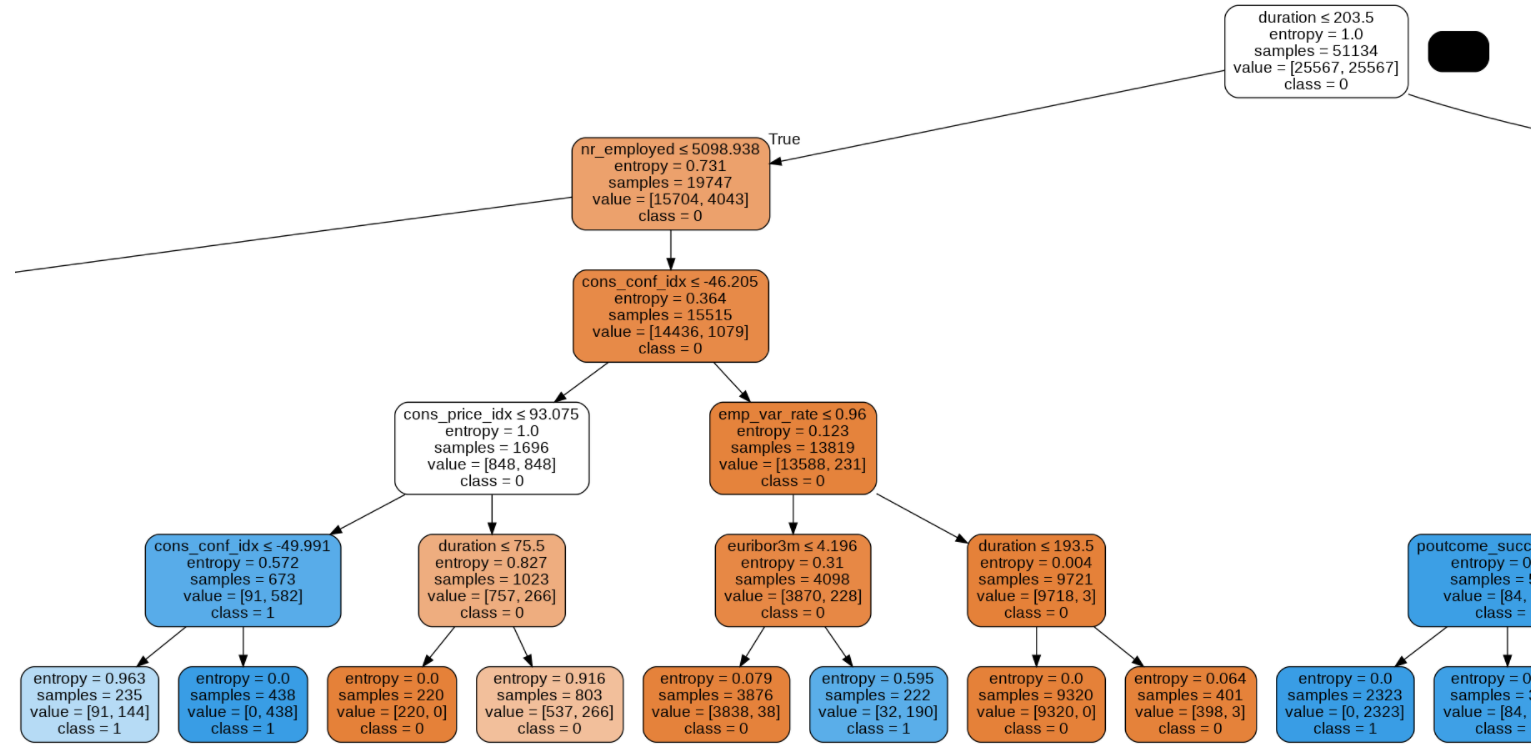
\includegraphics[scale =0.45]{images/tree_gra_smo.PNG}
    	\end{center}
    		\caption{Hình ảnh một phần của cây quyết định với tập dữ liệu cân bằng}
    \end{figure}
        \end{center} 
               \begin{itemize}
            \item Chọn thuộc tính duration làm gốc vì nó có giá trị Gain lớn nhất.
            \item samples ở đây chứa 51134 có nghĩa là cây này được training 28831 mẫu dữ liệu.
            \item Value [25567, 25567] là giá trị lớp mẫu, tức là có 25567 thuộc lớp 0, còn lại phân vào lớp 1. Hai giá trị bằng nhau phân gốc này thành lớp 0.
            \item So sánh điều kiện với duration nếu đúng thì nó sẽ phân nhánh ra cây con mới bên trái.
    \end{itemize}
\item [- ]	Nhận xét:
     \begin{itemize}
            \item Dữ liệu khi tiến hành thực thi thuật toán ta thấy dữ liệu cân bằng với dữ liệu gốc có độ chính xác khá chênh lệch.
            \item Độ chính xác của thuật toán với tập dữ liệu gốc cao hơn so với tập dữ liệu được cân bằng.
            \item Tính đến thời điểm này, thì thuật toán Decision Tree thực nghiệm trên tập dữ liệu gốc có độ chính xác cao với thời gian chạy nhanh nhất so các thuật toán trước.
    \end{itemize}
    \end{enumerate}
    $\Rightarrow$ \textbf{Kết luận: }
    \begin{enumerate}
    \item [- ] Đối với tập dữ liệu gốc, sau khi trải qua 5 thuật toán thì ta thấy Decision Tree có thời gian chạy nhanh nhất và độ chính xác thấp hơn KNN 1\% nhưng thời gian chạy KNN lại lâu hơn.  
    \item [- ] Dối với tập dữ liệu được xử lý cân bằng, thuật toán LR có độ chính xác cao nhất. Thuật toán NB với độ chính xác 85\% cho ra kết quả nhanh nhất.
    \end{enumerate}
    
  %-------------------------------------------------------------------------------------------------------------
%---------------Chương 5 -----------------------
\fontsize{16}{10}\selectfont
\chapter{KẾT LUẬN}
\fontsize{14}{10}\selectfont
\section{Kết quả đạt được}
     \fontsize{13}{14}\selectfont
     \begin{enumerate}
     \item [- ] Thu thập và xử lý tập dữ liệu phù hợp cho việc nghiên cứu báo cáo.
    \item [- ] Thực hiện dự đoán với tập dữ liệu ngân hàng của dịch vụ khách hàng đăng ký tiền gửi có kỳ hạn.
    \item[- ] Đồ thị hóa với Tableau.
    \item [- ] Tìm hiểu 5 thuật toán và áp dụng các thuật toán ấy vào đề tài để đưa ra kết quả dự đoán.
    \end{enumerate}

\fontsize{14}{10}\selectfont
\section{Mặt hạn chế}
     \fontsize{13}{14}\selectfont
     Trong quá trình làm báo cáo, chúng em đã cố gắng nghiên cứu và tìm hiểu để có được những kết quả trên. Tuy nhiên do hạn chế về mặt kiến thức cũng như kĩ năng,mặt khác về một số điều kiện về thời gian và không gian, chúng em chưa thể sử dụng nhiều thuật toán khác để áp dụng. 

\fontsize{14}{10}\selectfont
\section{Hướng phát triển}
     \fontsize{13}{14}\selectfont
     Vì đề tài còn mang tính thực tế hơn nữa, có khả năng ứng dụng cao với các mục tiêu cho tương lai sau này như dùng các thuật toán học máy khác nhau để phân tích và dự đoán tìm ra các chiến thuật hiệu quả nhất trong chiến dịch tiếp thị ngân hàng ví dụ như dự đoán hành vi trả nợ đúng hạn của khách hàng, đăng ký dịch vụ thẻ tín dụng,... để đưa ra các chiến lược hiệu quả và mang đến lợi nhuận cao cho ngân hàng.


 %-------------------------------------------------------------------------------------------------------------
%---------------Chapter 6 -----------------------        
\fontsize{18}{10}\selectfont
\chapter{TÀI LIỆU THAM KHẢO}
        \fontsize{13}{14}\selectfont
        \begin{enumerate}
            \item Moro, S., Cortez, P., \& Rita, P. (2014). A data-driven approach to predict the success of bank telemarketing. Decision Support Systems, 62, 22-31.
            \item Draper, N. R., \& Smith, H. (1998). “Dummy” variables. Applied regression analysis, 299-325.
            \item Jason Brownlee. (2020).\href {https://machinelearningmastery.com/smote-oversampling-for-imbalanced-classification/}{ SMOTE for Imbalanced Classification with Python.} Machine Learning Mastery.
            \item Hadeer Hammad \& Min Zhou. (2020). \href {https://ichi.pro/vi/du-lieu-khong-can-bang-trong-phan-loai-giai-phap-chung-nghien-cuu-dien-hinh-24872928981015}{Dữ liệu không cân bằng trong phân loại: Giải pháp chung \& Nghiên cứu điển hình.} ICHI.PRO.
            \item huytuong010101. (2020). \href {https://codelearn.io/sharing/thuat-toan-k-nearest-neighbors-knn}{Thuật Toán K-Nearest Neighbors (KNN).} codelearn.io.
            \item HVIT CLAN. (2020). \href{https://hvitclan.vn/blog/bai-8-knn-k-nearest-neighbors-194}{Bài 8 - KNN (K-Nearest Neighbors).} hvitclan.vn.
            \item Kiến thức kinh tế. (2020). \href {https://vietnambiz.vn/thuat-toan-k-lang-gieng-gan-nhat-k-nearest-neighbor-knn-la-gi-2020022911113334.htm}{Thuật toán K láng giềng gần nhất (K-Nearest Neighbor - KNN) là gì?} vietnambiz.vn.
            \item BIGDATAUNI. (2021). \href {https://bigdatauni.com/tin-tuc/tong-quan-ve-logistic-regression-hoi-quy-logistic-phan-2.html}{Tổng quan về Logistic Regresstion - Phần 2.} bigdatauni.com
            \item BIGDATAUNI. (2021). \href {https://bigdatauni.com/tin-tuc/tong-quan-ve-logistic-regression-hoi-quy-logistic-phan-1.html}{Tổng quan về Logistic Regresstion - Phần 1.} bigdatauni.com.
            \item Blog Trí tuệ nhân tạo. (2019). \href{https://trituenhantao.io/kien-thuc/decision-tree/}{Cây Quyết Định (Decision Tree).} trituenhantao.io.
            \item ICHI.PRO. (2020). \href {https://ichi.pro/vi/5-ky-thuat-smote-de-lay-mau-qua-muc-cho-du-lieu-mat-can-bang-cua-ban-202401874961077}{5 kỹ thuật SMOTE để lấy mẫu quá mức cho dữ liệu mất cân bằng của bạn.} ichi.pro.
            \item Data Science Notebook. (2016). \href{ https://sites.google.com/site/datasciencenotebook1/binary-classification/kernel-methods}{Kernel Methods \& Non Linear SVM.} Binary Classification.
            \item VIBLO. (2020). \href{https://viblo.asia/p/gioi-thieu-ve-support-vector-machine-svm-6J3ZgPVElmB?fbclid=IwAR2CmZvQt0Ke_3-6liQslGTPMRzn3qUS0h1CGf0jbFGhtw22vPDgCAWVVfM}{Giới thiệu về Support Vector Machine (SVM).} viblo.asia.
            \item Data Science, Machine Learning. (2018). \href{https://1upnote.me/post/2018/11/ds-ml-naive-bayes/}{Naive Bayes Classification (NBC) là gì?.} 1upnote.me.
            \item vietnambiz. (2019). \href{https://vietnambiz.vn/bien-gia-dummy-variable-trong-phan-tich-hoi-qui-la-gi-20191216174659595.htm}{Biến giả (Dummy variable) trong phân tích hồi qui là gì?.} vietnambiz.vn.
        \end{enumerate}
\end{document}
